% !TeX program = tectonic
% !TeX root = main.tex
\documentclass[aspectratio=169,10pt]{beamer}

\usepackage[T1]{fontenc}
% Match the NeurIPS font convention: Times roman text, Helvetica sans text,
% and conventional LaTeX paper mathematics.
\renewcommand{\rmdefault}{ptm}
\renewcommand{\sfdefault}{phv}
\usefonttheme{professionalfonts}
\usepackage{amsmath,amssymb,mathtools}
\usepackage{booktabs}
\usepackage{graphicx}
\usepackage{animate}
\usepackage{qrcode}
\usepackage{tikz}
\usetikzlibrary{arrows.meta,calc,fit,positioning,shapes.geometric}

\definecolor{Ink}{HTML}{17243A}
\definecolor{BrandBlue}{HTML}{1E90FF}
\colorlet{Navy}{BrandBlue}
\colorlet{Blue}{BrandBlue}
\definecolor{Ice}{HTML}{E9EFF4}
\colorlet{Sky}{BrandBlue!44!white}
\colorlet{BrightSky}{BrandBlue}
\definecolor{Mist}{HTML}{F4F6F8}
\definecolor{Slate}{HTML}{64748B}
\colorlet{Azure}{BrandBlue!72!black}
\definecolor{TerrainLight}{HTML}{DCE8E5}
\definecolor{TerrainMid}{HTML}{AFC8C4}
\definecolor{TerrainDark}{HTML}{769E9A}
\definecolor{Trail}{HTML}{D89A43}
\definecolor{TrailDark}{HTML}{9E6424}
\definecolor{DiffusionLatent}{HTML}{7C3AED}

\setbeamercolor{normal text}{fg=Ink,bg=white}
\setbeamercolor{structure}{fg=Navy}
\setbeamercolor{frametitle}{fg=white,bg=Navy}
\setbeamercolor{block title}{fg=white,bg=Blue}
\setbeamercolor{block body}{fg=Ink,bg=Ice!55!white}
\setbeamercolor{alerted text}{fg=Azure}
\setbeamerfont{frametitle}{series=\bfseries,size=\large}
\setbeamertemplate{navigation symbols}{}
\setbeamertemplate{itemize item}{$\color{Blue}\blacktriangleright$}
\setbeamertemplate{itemize subitem}{$\color{Navy}\bullet$}
\setbeamertemplate{footline}{%
  \leavevmode%
  \hbox{%
    \begin{beamercolorbox}[wd=.075\paperwidth,ht=2.6ex,dp=1.1ex,center]{author in head/foot}%
      \raisebox{-0.65ex}[0pt][0pt]{
\includegraphics[height=4.2ex]{assets/logos/atari_lab.png}}%
    \end{beamercolorbox}%
    \begin{beamercolorbox}[wd=.785\paperwidth,ht=2.6ex,dp=1.1ex,leftskip=0.35em]{author in head/foot}%
      \color{Slate}\scriptsize From Variational Inference to Diffusion-Based Reinforcement Learning
    \end{beamercolorbox}%
    \begin{beamercolorbox}[wd=.14\paperwidth,ht=2.6ex,dp=1.1ex,center]{date in head/foot}%
      \color{Navy}\scriptsize\insertframenumber/\inserttotalframenumber
    \end{beamercolorbox}%
  }%
}

% Institutional marks stay in the margins: TUM in the frame-title bar and
% ATARI Lab in the footer. Plain title/section frames use \plainlogos below.
\addtobeamertemplate{frametitle}{}{%
  \begin{tikzpicture}[remember picture,overlay]
    \node[anchor=north east,fill=white,rounded corners=1.2pt,
          inner xsep=2.8pt,inner ysep=1.8pt]
      at ([xshift=-0.16cm,yshift=-0.10cm]current page.north east)
      {
\includegraphics[height=0.52cm]{assets/logos/tum_logo.png}};
  \end{tikzpicture}%
}

\newcommand{\plainlogos}{%
  \begin{tikzpicture}[remember picture,overlay]
    \node[anchor=north east,fill=white,rounded corners=1.2pt,
          inner xsep=2.8pt,inner ysep=1.8pt]
      at ([xshift=-0.16cm,yshift=-0.12cm]current page.north east)
      {
\includegraphics[height=0.58cm]{assets/logos/tum_logo.png}};
    \node[anchor=south west,fill=white,rounded corners=1.2pt,
          inner sep=2.0pt]
      at ([xshift=0.16cm,yshift=0.13cm]current page.south west)
      {
\includegraphics[height=0.78cm]{assets/logos/atari_lab.png}};
  \end{tikzpicture}%
}

\newcommand{\E}{\mathbb{E}}
\newcommand{\R}{\mathbb{R}}
\newcommand{\KL}{D_{\mathrm{KL}}}
\newcommand{\Normal}{\mathrm{N}}
\newcommand{\entropy}{\mathrm{H}}
\newcommand{\Tau}{\mathcal{T}}
\newcommand{\thetar}{\theta_r}
\newcommand{\given}{\,\middle|\,}
\newcommand{\stopgrad}{\operatorname{stopgrad}}

% Exact state/color mapping from the source figure's shared legend:
% DMERL/Rebuttal_NeuriPs/LatexPaper/Figures/Ablations/multi_histo.png.
\newcommand{\multimodalstatelegend}{%
  
\begin{tikzpicture}[x=1.18cm,y=1cm,font=\scriptsize,baseline]
    \node[anchor=east] at (-0.10,0) {\textbf{State (heading):}};
    \foreach \i/\heading/\hex in {
      0/0/00FFF6,1/45/004BFF,2/90/7200FF,3/135/FF00CF,
      4/180/FF0000,5/225/FFBD00,6/270/84FF00,7/315/00FF39}{%
      \definecolor{HeadingColor}{HTML}{\hex}
      \draw[HeadingColor,line width=1.8pt] (\i,0) -- (\i+0.22,0);
      \node[anchor=west,inner sep=2pt] at (\i+0.24,0) {$\heading^\circ$};
    }
    \draw[black,line width=1.8pt] (8,0) -- (8.22,0);
    \node[anchor=west,inner sep=2pt] at (8.24,0) {reward};
  \end{tikzpicture}%
}

% Compact, reusable robot-arm glyph for the robotics motivation drawings.
% Arguments: color, opacity, shoulder, elbow, wrist, tool, gripper rotation.
\newcommand{\drawrobotarm}[7]{%
  \draw[white,line width=7pt,opacity=0.90]
    (#3) -- (#4) -- (#5) -- (#6);
  \draw[#1,line width=4.0pt,opacity=#2]
    (#3) -- (#4) -- (#5) -- (#6);
  \node[circle,draw=#1,fill=white,opacity=#2,line width=1.1pt,
        minimum size=6.2pt,inner sep=0pt] at (#3) {};
  \node[circle,draw=#1,fill=white,opacity=#2,line width=1.1pt,
        minimum size=6.2pt,inner sep=0pt] at (#4) {};
  \node[circle,draw=#1,fill=white,opacity=#2,line width=1.1pt,
        minimum size=6.2pt,inner sep=0pt] at (#5) {};
  \node[circle,draw=#1,fill=white,opacity=#2,line width=1.1pt,
        minimum size=6.2pt,inner sep=0pt] at (#6) {};
  \begin{scope}[shift={(#6)},rotate=#7,opacity=#2]
    \draw[#1,line width=2.2pt] (0,0) -- (0.24,0);
    \draw[#1,line width=1.8pt]
      (0.24,-0.16) -- (0.24,0.16)
      (0.24,0.16) -- (0.52,0.09)
      (0.24,-0.16) -- (0.52,-0.09);
  \end{scope}%
}

\newcommand{\drawrobotbase}[2]{%
  \path[fill=Slate!24,draw=Slate!62,rounded corners=1.5pt]
    ({#1-0.38},{#2-0.28}) rectangle ({#1+0.38},{#2});
  \path[fill=Slate!38,draw=Slate!68]
    ({#1-0.25},{#2}) -- ({#1+0.25},{#2})
    -- ({#1+0.17},{#2+0.34}) -- ({#1-0.17},{#2+0.34}) -- cycle;
}

\title{From Variational Inference to Diffusion-Based Reinforcement Learning}
\subtitle{}
\author{Sebastian Sanokowski}
\institute{Applied and Theoretical Aspects of Robot Intelligence Lab (ATARI)}
\date{}

\begin{document}

% The opening slide intentionally combines the title and the full talk trajectory.
\begin{frame}[plain]
  \plainlogos
  \vspace{0.56cm}
  \begin{center}
    \resizebox{0.90\textwidth}{!}{%
      \color{Ink}\bfseries
      From Variational Inference to Diffusion-Based Reinforcement Learning}
  \end{center}
  \vspace{0.14cm}
  \begin{center}
    {\large\bfseries\color{BrandBlue} Sebastian Sanokowski}\\[0.06cm]
    {\small\color{Slate}
      Applied and Theoretical Aspects of Robot Intelligence Lab (ATARI)}
  \end{center}

  \vfill
  \begin{center}
  \resizebox{0.96\textwidth}{!}{%
  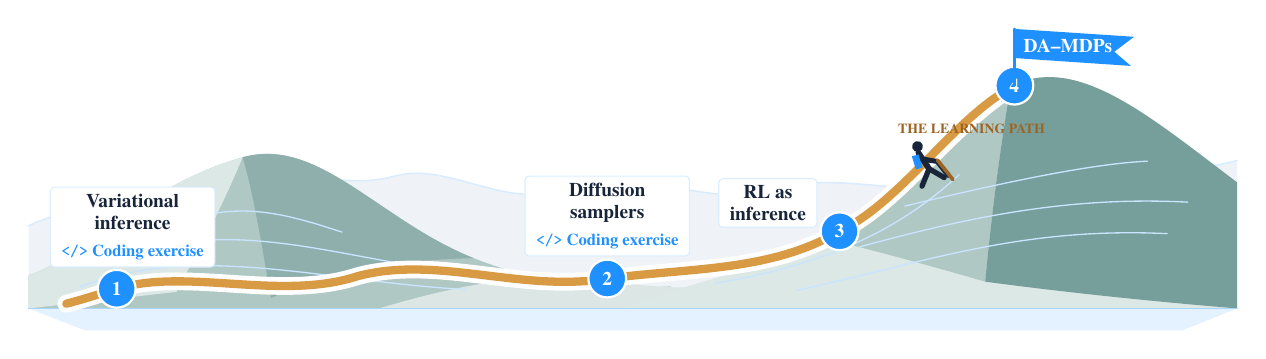
\begin{tikzpicture}[font=\sffamily,line cap=round,line join=round]
    % A distant ridge establishes depth without competing with the lesson path.
    \path[fill=Ice!72!white]
      (0,0.35) -- (0,1.35)
      .. controls (0.9,1.75) and (1.45,1.60) .. (2.15,1.92)
      .. controls (3.00,2.31) and (3.80,1.75) .. (4.65,1.98)
      .. controls (5.35,2.17) and (6.05,1.53) .. (6.90,1.82)
      .. controls (7.80,2.12) and (8.58,1.58) .. (9.38,1.80)
      .. controls (10.35,2.07) and (11.12,1.67) .. (12.05,1.90)
      .. controls (13.15,2.18) and (14.10,1.85) .. (15.35,2.18)
      -- (15.35,0.35) -- cycle;
    \draw[Sky!38,line width=0.55pt]
      (0,1.35)
      .. controls (0.9,1.75) and (1.45,1.60) .. (2.15,1.92)
      .. controls (3.00,2.31) and (3.80,1.75) .. (4.65,1.98)
      .. controls (5.35,2.17) and (6.05,1.53) .. (6.90,1.82)
      .. controls (7.80,2.12) and (8.58,1.58) .. (9.38,1.80)
      .. controls (10.35,2.07) and (11.12,1.67) .. (12.05,1.90)
      .. controls (13.15,2.18) and (14.10,1.85) .. (15.35,2.18);

    % Low hill, valley, and the final climb: broad shaded facets give a
    % hand-drawn isometric / 3-D feel while retaining the deck's muted palette.
    \path[fill=TerrainMid]
      (0,0.30) -- (0,0.72)
      .. controls (0.85,1.02) and (1.42,1.85) .. (2.72,2.22)
      .. controls (3.68,2.49) and (4.45,1.42) .. (5.65,0.94)
      .. controls (6.45,0.62) and (7.30,0.54) .. (8.15,0.58)
      -- (8.48,0.30) -- cycle;
    \path[fill=TerrainLight]
      (0,0.72)
      .. controls (0.85,1.02) and (1.42,1.85) .. (2.72,2.22)
      .. controls (2.37,1.38) and (2.08,0.91) .. (1.88,0.51)
      -- (0,0.30) -- cycle;
    \path[fill=TerrainDark!82!white]
      (2.72,2.22)
      .. controls (3.68,2.49) and (4.45,1.42) .. (5.65,0.94)
      .. controls (4.65,0.91) and (3.75,0.77) .. (3.08,0.43)
      .. controls (2.95,1.17) and (2.86,1.74) .. (2.72,2.22) -- cycle;

    \path[fill=TerrainDark!26!white]
      (4.45,0.30)
      .. controls (5.80,0.70) and (6.58,0.77) .. (7.62,0.62)
      .. controls (8.48,0.49) and (9.05,0.61) .. (9.78,0.89)
      .. controls (10.36,1.12) and (10.78,1.42) .. (11.18,1.72)
      -- (11.92,0.30) -- cycle;
    \path[fill=TerrainLight]
      (7.58,0.30)
      .. controls (8.62,0.72) and (9.38,0.80) .. (10.15,1.18)
      .. controls (10.87,1.54) and (11.42,2.58) .. (12.47,3.12)
      .. controls (13.30,3.54) and (14.20,2.77) .. (15.35,1.90)
      -- (15.35,0.30) -- cycle;
    \path[fill=TerrainMid]
      (10.15,1.18)
      .. controls (10.87,1.54) and (11.42,2.58) .. (12.47,3.12)
      .. controls (12.35,2.36) and (12.25,1.69) .. (12.15,0.64)
      .. controls (11.46,0.84) and (10.84,1.01) .. (10.15,1.18) -- cycle;
    \path[fill=TerrainDark]
      (12.47,3.12)
      .. controls (13.30,3.54) and (14.20,2.77) .. (15.35,1.90)
      -- (15.35,0.30)
      .. controls (14.15,0.40) and (13.13,0.51) .. (12.15,0.64)
      .. controls (12.25,1.69) and (12.35,2.36) .. (12.47,3.12) -- cycle;

    % Front edge and sparse contours reinforce the perspective-sketch effect.
    \path[fill=Navy!12]
      (0,0.30) -- (15.35,0.30) -- (14.65,0.02) -- (0.72,0.02) -- cycle;
    \draw[Navy!38,line width=0.6pt] (0,0.30) -- (15.35,0.30);
    \draw[Navy!24,line width=0.48pt]
      (0.65,0.57) .. controls (2.15,1.15) and (3.72,0.64) .. (5.56,0.54);
    \draw[Navy!24,line width=0.48pt]
      (1.13,0.89) .. controls (2.28,1.43) and (3.55,1.07) .. (4.78,0.86);
    \draw[Navy!24,line width=0.48pt]
      (1.72,1.30) .. controls (2.58,1.72) and (3.27,1.50) .. (3.98,1.27);
    \draw[Navy!24,line width=0.48pt]
      (8.72,0.62) .. controls (10.22,0.87) and (11.12,1.35) .. (11.82,2.00);
    \draw[Navy!24,line width=0.48pt]
      (9.76,0.53) .. controls (11.34,0.87) and (12.57,1.34) .. (14.46,1.25);
    \draw[Navy!24,line width=0.48pt]
      (10.55,1.08) .. controls (11.90,1.45) and (13.20,1.73) .. (14.72,1.65);
    \draw[Navy!24,line width=0.48pt]
      (11.13,1.60) .. controls (12.42,1.91) and (13.52,2.14) .. (14.21,2.17);

    % The curriculum is one continuous trail through the landscape.
    \coordinate (m1) at (1.12,0.55);
    \coordinate (m2) at (4.18,0.71);
    \coordinate (m3) at (7.35,0.68);
    \coordinate (m4) at (10.30,1.28);
    \coordinate (m5) at (12.52,3.13);
    \draw[white!88,line width=6.4pt]
      (0.48,0.36)
      .. controls (0.82,0.45) and (0.94,0.50) .. (m1)
      .. controls (2.02,0.82) and (3.20,0.39) .. (m2)
      .. controls (5.20,0.98) and (6.25,0.50) .. (m3)
      .. controls (8.44,0.82) and (9.43,0.77) .. (m4)
      .. controls (11.05,1.64) and (11.70,2.63) .. (m5);
    \draw[Trail,line width=3.0pt,-{Stealth[length=7pt,width=5pt]}]
      (0.48,0.36)
      .. controls (0.82,0.45) and (0.94,0.50) .. (m1)
      .. controls (2.02,0.82) and (3.20,0.39) .. (m2)
      .. controls (5.20,0.98) and (6.25,0.50) .. (m3)
      .. controls (8.44,0.82) and (9.43,0.77) .. (m4)
      .. controls (11.05,1.64) and (11.70,2.63) .. (m5);

    % Milestones sit directly on the trail; compact white signboards preserve
    % legibility over the shaded terrain.
    \foreach \name/\num in {m1/1,m3/2,m4/3,m5/4}{
      \node[circle,fill=Navy,draw=white,line width=0.8pt,minimum size=4.8mm,
            inner sep=0pt,text=white,font=\bfseries\scriptsize] at (\name) {\num};
    }
    \node[fill=white,draw=Navy!16,rounded corners=1.5pt,inner xsep=4pt,
          inner ysep=2.4pt,align=center,text=Ink,font=\bfseries\scriptsize,
          anchor=south west] at (0.27,0.82)
          {Variational\\inference\\[2pt]
           {\color{BrandBlue}\fontsize{6}{7}\selectfont
            \texttt{</>} Coding exercise}};
    \node[fill=white,draw=Navy!16,rounded corners=1.5pt,inner xsep=4pt,
          inner ysep=2.4pt,align=center,text=Ink,font=\bfseries\scriptsize,
          anchor=south] at (7.35,0.96)
          {Diffusion\\samplers\\[2pt]
           {\color{BrandBlue}\fontsize{6}{7}\selectfont
            \texttt{</>} Coding exercise}};
    \node[fill=white,draw=Navy!16,rounded corners=1.5pt,inner xsep=4pt,
          inner ysep=2.4pt,align=center,text=Ink,font=\bfseries\scriptsize,
          anchor=east] at (10.02,1.64) {RL as\\inference};

    % Summit flag: the final lesson is the destination of the climb.
    \draw[Navy,line width=0.9pt] (m5) -- ++(0,0.72);
    \path[fill=Navy]
      ($(m5)+(0,0.72)$) -- ($(m5)+(1.52,0.62)$)
      -- ($(m5)+(1.27,0.43)$) -- ($(m5)+(1.48,0.25)$)
      -- ($(m5)+(0,0.35)$) -- cycle;
    \node[text=white,font=\bfseries\scriptsize,anchor=center]
      at ($(m5)+(0.68,0.50)$) {DA--MDPs};

    % A small hiker, leaning into the last ascent.
    \begin{scope}[shift={(11.35,2.12)},rotate=17,scale=0.58]
      \fill[Ink] (0.02,0.42) circle (0.12);
      \draw[Ink,line width=2.1pt] (0.00,0.28) -- (0.12,-0.12);
      \draw[Ink,line width=1.8pt] (0.06,0.12) -- (0.34,-0.02);
      \draw[Ink,line width=1.8pt] (0.34,-0.02) -- (0.48,-0.38);
      \draw[Ink,line width=1.9pt] (0.12,-0.12) -- (0.38,-0.40);
      \draw[Ink,line width=1.9pt] (0.12,-0.12) -- (-0.14,-0.44);
      \path[fill=Blue] (-0.16,0.25) rectangle (-0.01,-0.05);
      \draw[TrailDark,line width=1.3pt] (0.35,0.01) -- (0.55,-0.50);
    \end{scope}
    \node[text=TrailDark,font=\bfseries\tiny,anchor=south west]
      at (10.92,2.40) {THE LEARNING PATH};
  \end{tikzpicture}}
  \end{center}
\end{frame}

{
\setbeamercolor{frametitle}{fg=white,bg=BrandBlue}
\setbeamercolor{block title}{fg=white,bg=BrandBlue}
\setbeamercolor{block body}{fg=Ink,bg=BrandBlue!8!white}
\setbeamercolor{structure}{fg=BrandBlue}

\begin{frame}{A robotics task can have multiple valid solutions}
  \centering
  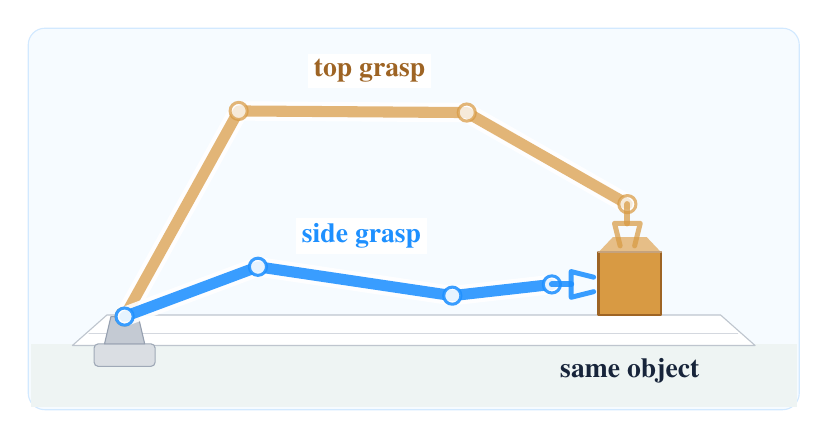
\begin{tikzpicture}[x=1.02cm,y=1.02cm,font=\small,
      line cap=round,line join=round]
    \path[fill=BrandBlue!4,draw=Navy!20,rounded corners=6pt]
      (0,0) rectangle (9.6,4.75);
    \path[fill=TerrainLight!48!white]
      (0.03,0.03) rectangle (9.57,0.82);
    \path[fill=white,draw=Slate!42]
      (0.55,0.80) -- (9.05,0.80) -- (8.62,1.18) -- (0.98,1.18) -- cycle;
    \draw[Slate!28,line width=0.6pt] (0.76,0.95) -- (8.83,0.95);
    \uncover<1->{%
      \drawrobotbase{1.20}{0.82}
      \path[fill=Trail,draw=TrailDark,line width=0.8pt]
        (7.10,1.18) rectangle (7.88,1.96);
      \path[fill=Trail!64!white]
        (7.10,1.96) -- (7.88,1.96) -- (7.70,2.15) -- (7.28,2.15) -- cycle;
      \draw[TrailDark!60,line width=0.6pt] (7.10,1.96) -- (7.88,1.96);
      \node[text=Ink,font=\bfseries] at (7.49,0.48) {same object};
    }
    \uncover<2->{%
      \drawrobotarm{Trail}{0.72}{1.20,1.16}{2.62,3.72}{5.46,3.70}{7.46,2.56}{-90}
      \node[text=TrailDark,font=\bfseries,fill=white,inner sep=2pt]
        at (4.25,4.22) {top grasp};
    }
    \uncover<3->{%
      \drawrobotarm{BrandBlue}{0.88}{1.20,1.16}{2.86,1.78}{5.28,1.42}{6.52,1.56}{0}
      \node[text=BrandBlue,font=\bfseries,fill=white,inner sep=2pt]
        at (4.15,2.16) {side grasp};
    }
  \end{tikzpicture}
\end{frame}

\begin{frame}{What multimodality buys us}
  % Keep the institutional mark visible on the first reveal state as well.
  \only<1>{%
    \begin{tikzpicture}[remember picture,overlay]
      \node[anchor=north east,fill=white,rounded corners=1.2pt,
            inner xsep=2.8pt,inner ysep=1.8pt]
        at ([xshift=-0.16cm,yshift=-0.10cm]current page.north east)
        {
\includegraphics[height=0.52cm]{assets/logos/tum_logo.png}};
    \end{tikzpicture}%
  }
  \begin{columns}[T,onlytextwidth]
    \column{0.32\textwidth}
      \centering
      \uncover<1->{%
      {\bfseries\color{Ink}Better exploration}\par\vspace{0.12cm}
      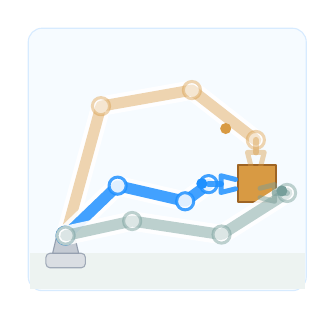
\begin{tikzpicture}[x=0.66cm,y=0.66cm,line cap=round,line join=round]
        \path[fill=BrandBlue!4,draw=Navy!18,rounded corners=5pt]
          (0,0) rectangle (5.35,5.05);
        \path[fill=TerrainLight!52!white]
          (0.03,0.03) rectangle (5.32,0.72);
        \drawrobotbase{0.72}{0.72}
        \path[fill=Trail,draw=TrailDark,line width=0.7pt]
          (4.04,1.70) rectangle (4.76,2.42);
        \drawrobotarm{Trail}{0.42}{0.72,1.06}{1.40,3.55}{3.15,3.86}{4.38,2.90}{-90}
        \drawrobotarm{BrandBlue}{0.84}{0.72,1.06}{1.72,2.02}{3.02,1.72}{3.47,2.05}{0}
        \drawrobotarm{TerrainDark}{0.48}{0.72,1.06}{2.00,1.34}{3.72,1.08}{4.98,1.88}{180}
        \foreach \x/\y/\c in {3.80/3.12/Trail,3.34/2.06/BrandBlue,
          4.88/1.92/TerrainDark}{\fill[\c] (\x,\y) circle (2.0pt);}
      \end{tikzpicture}}

    \column{0.32\textwidth}
      \centering
      \uncover<2->{%
      {\bfseries\color{Ink}Better adaptability}\par\vspace{0.12cm}
      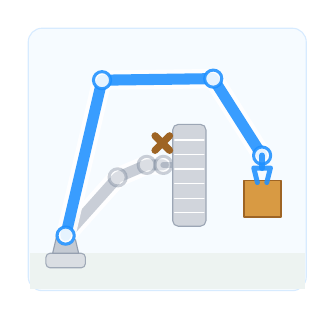
\begin{tikzpicture}[x=0.66cm,y=0.66cm,line cap=round,line join=round]
        \path[fill=BrandBlue!4,draw=Navy!18,rounded corners=5pt]
          (0,0) rectangle (5.35,5.05);
        \path[fill=TerrainLight!52!white]
          (0.03,0.03) rectangle (5.32,0.72);
        \drawrobotbase{0.72}{0.72}
        \path[fill=Trail,draw=TrailDark,line width=0.7pt]
          (4.16,1.42) rectangle (4.86,2.12);
        \drawrobotarm{Slate}{0.34}{0.72,1.06}{1.72,2.18}{2.28,2.42}{2.60,2.42}{0}
        \path[fill=Slate!30,draw=Slate!64,rounded corners=2pt]
          (2.78,1.24) rectangle (3.42,3.20);
        \foreach \y in {1.50,1.78,2.06,2.34,2.62,2.90}{
          \draw[white!78,line width=0.45pt] (2.82,\y) -- (3.38,\y);
        }
        \draw[TrailDark,line width=2.6pt]
          (2.44,2.70) -- (2.72,2.98)
          (2.72,2.70) -- (2.44,2.98);
        \drawrobotarm{BrandBlue}{0.88}{0.72,1.06}{1.42,4.05}{3.56,4.08}{4.50,2.60}{-90}
      \end{tikzpicture}}

    \column{0.32\textwidth}
      \centering
      \uncover<3->{%
      {\bfseries\color{Ink}Better world model}\par\vspace{0.12cm}
      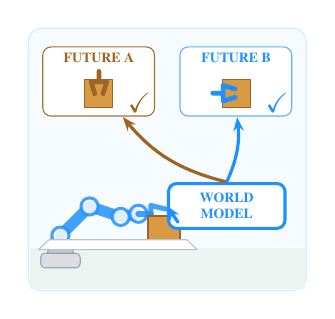
\begin{tikzpicture}[x=0.66cm,y=0.66cm,line cap=round,line join=round]
        \path[fill=BrandBlue!4,draw=Navy!18,rounded corners=5pt]
          (0,0) rectangle (5.35,5.05);
        \path[fill=TerrainLight!52!white]
          (0.03,0.03) rectangle (5.32,0.82);

        % The observed robotics scene.
        \drawrobotbase{0.62}{0.72}
        \drawrobotarm{BrandBlue}{0.84}{0.62,1.06}{1.18,1.62}{1.78,1.42}{2.12,1.48}{0}
        \path[fill=Trail,draw=TrailDark,line width=0.7pt]
          (2.30,0.82) rectangle (2.92,1.44);
        \path[fill=white,draw=Slate!44]
          (0.20,0.79) -- (3.25,0.79) -- (3.05,0.98) -- (0.40,0.98) -- cycle;

        % A learned model maps the scene to two distinct successful futures.
        \node[draw=BrandBlue,fill=white,rounded corners=3pt,line width=1.1pt,
              text=BrandBlue,font=\bfseries\tiny,minimum width=1.48cm,
              minimum height=0.50cm,align=center] (model) at (3.82,1.63)
          {WORLD\\MODEL};
        \draw[-{Stealth[length=5pt]},BrandBlue,line width=1.2pt]
          (2.88,1.32) -- (model.west);

        \path[fill=white,draw=Trail!75!black,rounded corners=3pt]
          (0.28,3.36) rectangle (2.43,4.69);
        \path[fill=white,draw=BrandBlue!70,rounded corners=3pt]
          (2.92,3.36) rectangle (5.07,4.69);
        \node[text=TrailDark,font=\bfseries\tiny] at (1.36,4.48) {FUTURE A};
        \node[text=BrandBlue,font=\bfseries\tiny] at (4.00,4.48) {FUTURE B};
        \path[fill=Trail,draw=TrailDark] (1.09,3.52) rectangle (1.63,4.06);
        \path[fill=Trail,draw=TrailDark] (3.73,3.52) rectangle (4.27,4.06);
        \begin{scope}[shift={(1.36,4.22)},rotate=-90]
          \draw[TrailDark,line width=1.7pt]
            (0,0)--(0.20,0) (0.20,-0.15)--(0.20,0.15)
            (0.20,0.15)--(0.43,0.08) (0.20,-0.15)--(0.43,-0.08);
        \end{scope}
        \begin{scope}[shift={(3.55,3.80)}]
          \draw[BrandBlue,line width=1.7pt]
            (0,0)--(0.20,0) (0.20,-0.15)--(0.20,0.15)
            (0.20,0.15)--(0.43,0.08) (0.20,-0.15)--(0.43,-0.08);
        \end{scope}
        \node[text=TrailDark,font=\bfseries] at (2.14,3.62) {$\checkmark$};
        \node[text=BrandBlue,font=\bfseries] at (4.79,3.62) {$\checkmark$};

        \draw[-{Stealth[length=5pt]},TrailDark,line width=1.15pt]
          (model.north) to[bend left=18] (1.82,3.34);
        \draw[-{Stealth[length=5pt]},BrandBlue,line width=1.15pt]
          (model.north) to[bend right=15] (4.02,3.34);
      \end{tikzpicture}}
  \end{columns}
\end{frame}

% Keep the paper link available throughout both multimodal demonstrations.
\newcommand{\damdppapercard}{%
  \centering
  {\small\bfseries\color{BrandBlue}DA-MDP paper}\par
  \vspace{0.15cm}
  \href{https://arxiv.org/abs/2512.02019}{%
    \qrcode[height=1.90cm]{https://arxiv.org/abs/2512.02019}}
  \par\vspace{0.14cm}
  \begin{itemize}
    \item \scriptsize Updated version in about 2 weeks.
  \end{itemize}
}

\begin{frame}{StackCube: one symmetric task, two solution modes}
  \begin{columns}[c,onlytextwidth]
    \column{0.76\textwidth}
      \centering
      \animategraphics[autoplay,loop,poster=last,height=0.69\textheight]
        {5}{assets/stackcube_overlay/frame-}{0}{22}
    \column{0.21\textwidth}
      \damdppapercard
  \end{columns}
  \vspace{0.08cm}
  \begin{itemize}
    \item \small Same initial scene, two valid stacking orders; \textbf{DA:REPPO}.
  \end{itemize}
\end{frame}

\begin{frame}{PushT: one initial state, two rotation modes}
  \begin{columns}[c,onlytextwidth]
    \column{0.76\textwidth}
      \centering
      \makebox[0.5\linewidth]{\bfseries Clockwise}%
      \makebox[0.5\linewidth]{\bfseries Counter-clockwise}\par
      \vspace{0.10cm}
      \animategraphics[autoplay,loop,poster=26,width=\linewidth]
        {10}{assets/pusht_multimodal/frame-}{0}{116}
    \column{0.21\textwidth}
      \damdppapercard
  \end{columns}
  \vspace{0.08cm}
  \begin{itemize}
    \item \small Same initial state ($192^\circ$), same \textbf{DA:REPPO} policy.
    \item \small Different diffusion-prior samples $\to$ two successful strategies.
  \end{itemize}
\end{frame}
}

\section{Lesson 1: Variational inference}

\begin{frame}[plain]
  \begin{tikzpicture}[remember picture,overlay]
    \fill[Navy] (current page.south west) rectangle (current page.north east);
    \fill[Sky] (current page.south west) rectangle
      ([xshift=1.3cm]current page.north west);
    \node[anchor=center,text=white,align=center]
      at ([xshift=0.65cm]current page.center)
      {{\bfseries\fontsize{16}{18}\selectfont LESSON 1}\\[0.24cm]
       {\bfseries\fontsize{25}{28}\selectfont Variational Inference}};
  \end{tikzpicture}
  \plainlogos
\end{frame}

\begin{frame}{Variational inference: from cost to a target distribution}
  \footnotesize
  \setlength{\abovedisplayskip}{4pt}
  \setlength{\belowdisplayskip}{4pt}
  \begin{columns}[c,onlytextwidth]
    \column{0.46\textwidth}
      \begin{itemize}
        \setlength{\itemsep}{0.26cm}
        \item<1-> \textbf{Given:} cost $\textcolor{TrailDark}{C(x)}$; lower is better.
        \item<2-> \textbf{Boltzmann target} ($\Tau>0$):
          \[
            \textcolor{TrailDark}{p_{\Tau}}(x)=\frac{e^{-\textcolor{TrailDark}{C(x)}/\Tau}}{Z_{\Tau}},
          \]
          \[
            Z_{\Tau}=\int e^{-\textcolor{TrailDark}{C(x)}/\Tau}\,dx<\infty.
          \]
        \item<3-> \textbf{Approximate} $\textcolor{TrailDark}{p_{\Tau}}$ with tractable
          $\textcolor{BrandBlue}{q_\theta}$ (e.g., a Gaussian).
        \item<4-> \textbf{Fit} $\textcolor{BrandBlue}{q_\theta}$ by minimizing its KL divergence
          to $\textcolor{TrailDark}{p_{\Tau}}$.
      \end{itemize}
    \column{0.52\textwidth}
      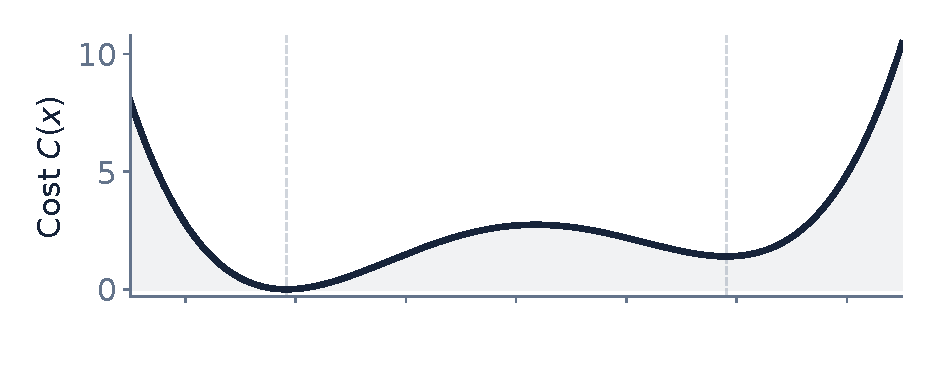
\includegraphics[width=\linewidth]{assets/boltzmann_cost.pdf}

      \uncover<2->{%
        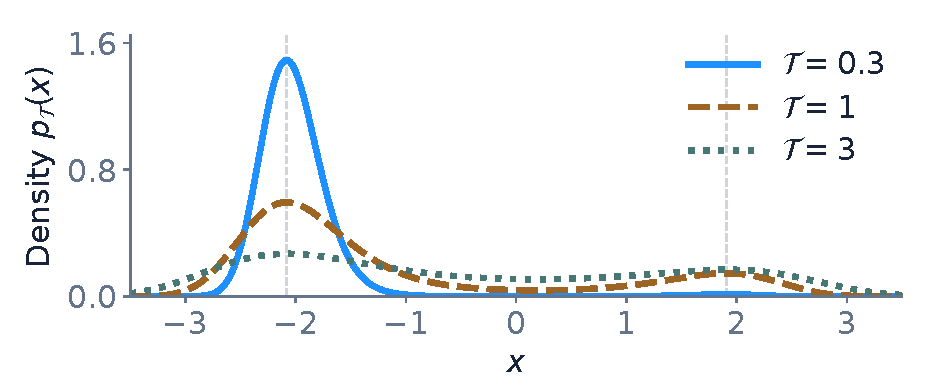
\includegraphics[width=\linewidth]{assets/boltzmann_temperatures.pdf}}
  \end{columns}
\end{frame}

\begin{frame}{Kullback--Leibler (KL) divergence}
  \footnotesize
  \setlength{\abovedisplayskip}{3pt}
  \setlength{\belowdisplayskip}{3pt}
  \begin{itemize}
    \item<1-> \textbf{Integral $\rightarrow$ expectation:}
      \[
        \KL(\textcolor{TrailDark}{p}\|\textcolor{BrandBlue}{q})
        =\int \textcolor{TrailDark}{p(x)}\log\frac{\textcolor{TrailDark}{p(x)}}{\textcolor{BrandBlue}{q(x)}}\,dx
        =\E_{X\sim \textcolor{TrailDark}{p}}\!\left[\log\frac{\textcolor{TrailDark}{p(X)}}{\textcolor{BrandBlue}{q(X)}}\right].
      \]
    \item<2-> $\KL\geq0$; zero iff $p=q$ (a.e.); asymmetric; can be infinite.
    \item<3-> \textbf{Same target $p$, single-Gaussian approximation $q_\theta$:}
  \end{itemize}
  \vspace{0.06cm}

  \uncover<3->{%
    \begin{columns}[T,onlytextwidth]
      \column{0.49\textwidth}
        \begin{itemize}
          \item \textbf{Forward: mode covering}
            \quad $\min_\theta\KL(\textcolor{TrailDark}{p}\|\textcolor{BrandBlue}{q_\theta})$
        \end{itemize}
        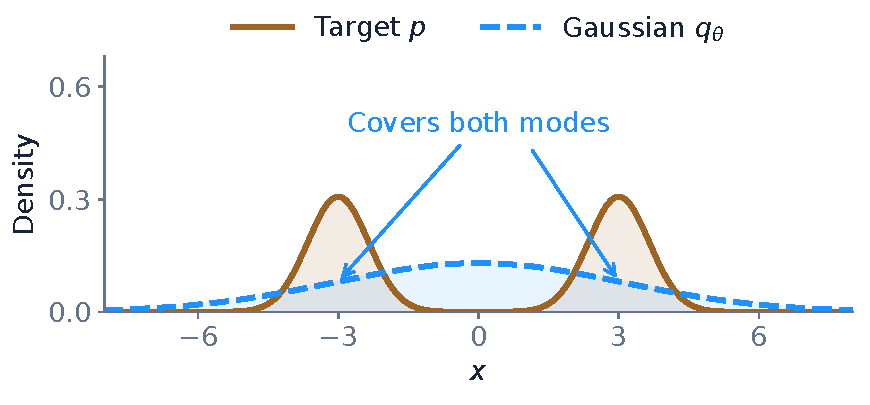
\includegraphics[width=\linewidth]{assets/kl_forward.pdf}
      \column{0.49\textwidth}
        \begin{itemize}
          \item \textbf{Reverse: mode seeking}
            \quad $\min_\theta\KL(\textcolor{BrandBlue}{q_\theta}\|\textcolor{TrailDark}{p})$
        \end{itemize}
        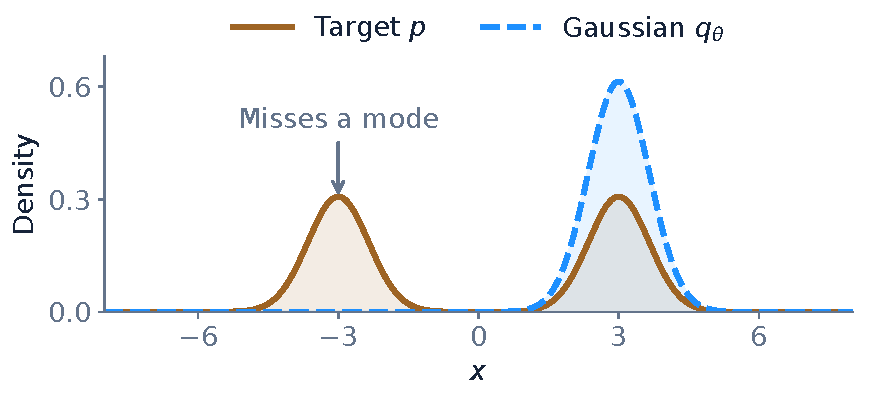
\includegraphics[width=\linewidth]{assets/kl_reverse.pdf}
    \end{columns}
    \begin{itemize}
      \item \textbf{Our VI objective:} $\min_\theta\KL(\textcolor{BrandBlue}{q_\theta}\|\textcolor{TrailDark}{p_{\Tau}})$.
    \end{itemize}
  }
\end{frame}

\begin{frame}{From variational inference to reward maximization}
  \small
  \begin{block}<1->{Expand the reverse KL: reward $R(x)=-C(x)$, $\Tau>0$}
    \[
      \begin{aligned}
      \Tau\KL(\textcolor{BrandBlue}{q_\theta}\|\textcolor{TrailDark}{p_{\Tau}})
      &=\Tau\E_{X\sim q_\theta}\!\left[
          \textcolor{BrandBlue}{\log q_\theta(X)}-\frac{\textcolor{TrailDark}{R(X)}}{\Tau}+\log Z_{\Tau}
        \right]\\
      &=-\underbrace{\left(
          \E_{X\sim q_\theta}\!\left[\textcolor{TrailDark}{R(X)}\right]
          +\textcolor{BrandBlue}{\Tau\mathcal H[q_\theta]}
        \right)}_{J_{\Tau}(\theta)}
        +\textcolor{Slate}{\Tau\log Z_{\Tau}}.
      \end{aligned}
    \]
  \end{block}

  \begin{alertblock}<2->{The optimization objective}
    \[
      \boxed{%
      \min_\theta\KL(\textcolor{BrandBlue}{q_\theta}\|\textcolor{TrailDark}{p_{\Tau}})
      \quad\Longleftrightarrow\quad
      \max_\theta J_{\Tau}(\theta)
      =\max_\theta\left(
        \E_{q_\theta}\!\left[\textcolor{TrailDark}{R(X)}\right]
        +\textcolor{BrandBlue}{\Tau\mathcal H[q_\theta]}
      \right).}
    \]
  \end{alertblock}

  \uncover<3->{%
    \begin{center}
      \textbf{Zero-temperature limit:}\qquad
      $J_0(\theta):=\displaystyle\lim_{\Tau\downarrow0}J_{\Tau}(\theta)
      =\E_{X\sim q_\theta}\!\left[\textcolor{TrailDark}{R(X)}\right]$.
      \\[0.10cm]
      Reward maximization is variational inference with the entropy term removed.
    \end{center}
  }
\end{frame}

\begin{frame}{Reparameterization trick: a Gaussian example}
  \footnotesize
  \setlength{\abovedisplayskip}{4pt}
  \setlength{\belowdisplayskip}{4pt}
  \begin{itemize}[<+->]
    \item \textbf{Start with a Gaussian:}
      \[
        q_\theta=\Normal(\textcolor{BrandBlue}{\mu},\textcolor{BrandBlue}{\sigma}^2),
        \qquad \theta=(\textcolor{BrandBlue}{\mu},\textcolor{BrandBlue}{\sigma}),\quad \textcolor{BrandBlue}{\sigma}>0.
      \]
    \item \textbf{Sample standard noise, then shift and scale:}
      \[
        \textcolor{Slate}{\varepsilon_i}\sim\Normal(0,1),
        \qquad \boxed{X_i=\textcolor{BrandBlue}{\mu}+\textcolor{BrandBlue}{\sigma}\textcolor{Slate}{\varepsilon_i}\sim q_\theta.}
      \]
    \item \textbf{Hold $\textcolor{Slate}{\varepsilon_i}$ fixed during backpropagation:}
      for differentiable $R$,
      \[
        \frac{\partial R(X_i)}{\partial\textcolor{BrandBlue}{\mu}}=R'(X_i),
        \qquad
        \frac{\partial R(X_i)}{\partial\textcolor{BrandBlue}{\sigma}}
        =R'(X_i)\,\textcolor{Slate}{\varepsilon_i}.
      \]
    \item \textbf{Gaussian VI loss} (samples via \texttt{q.rsample()}):
      \[
        \boxed{\widehat L_{\mathrm{path}}
        =-\frac1N\sum_{i=1}^{N}R(\textcolor{BrandBlue}{\mu}+\textcolor{BrandBlue}{\sigma}\textcolor{Slate}{\varepsilon_i})
         -\Tau\underbrace{\tfrac12\log(2\pi e\textcolor{BrandBlue}{\sigma}^2)}_{
           \text{Gaussian entropy }\mathcal H[q_\theta]}.}
      \]
  \end{itemize}
\end{frame}

\begin{frame}{Log-derivative trick for variational inference}
  \footnotesize
  \setlength{\abovedisplayskip}{4pt}
  \setlength{\belowdisplayskip}{4pt}
  \begin{itemize}[<+->]
    \item Differentiate the density instead of the sampled value:
      \[
        \nabla_\theta J_{\Tau}
        =\E_{X\sim q_\theta}\!\left[
          \left(\textcolor{TrailDark}{R(X)}-\textcolor{BrandBlue}{\Tau\log q_\theta(X)}-b\right)
          \textcolor{BrandBlue}{\nabla_\theta\log q_\theta(X)}
        \right].
      \]
    \item A leave-one-out baseline keeps the estimator unbiased:
      \[
        S_i=\textcolor{TrailDark}{R(X_i)}-\textcolor{BrandBlue}{\Tau\log q_\theta(X_i)},
        \qquad
        b_i=\frac{1}{N-1}\sum_{j\neq i}S_j.
      \]
    \item Use the detached learning signal in the Monte Carlo loss:
      \[
        \boxed{\widehat L_{\mathrm{score}}
        =-\frac1N\sum_{i=1}^{N}
          \textcolor{Slate}{\stopgrad(S_i-b_i)}\textcolor{BrandBlue}{\log q_\theta(X_i)}.}
      \]
  \end{itemize}
  \uncover<4->{\scriptsize
    Only $\log q_\theta(X)$ must be differentiable: $\textcolor{TrailDark}{R(X)}$ may be a black box,
    at the cost of typically higher variance.}
\end{frame}

\begin{frame}{Lesson 1 exercise: GMM-40 variational inference}
  \small
  \setlength{\abovedisplayskip}{3pt}
  \setlength{\belowdisplayskip}{3pt}
  \setlength{\jot}{2pt}
  \begin{columns}[T,onlytextwidth]
    \column{0.53\textwidth}
      \uncover<1->{%
        \begin{align*}
          \mu_i&\overset{\mathrm{iid}}{\sim}
            \operatorname{Unif}([-40,40]^2),\quad i=1,\ldots,40,\\
          \textcolor{TrailDark}{p_{\mathrm{ref}}}(x)
            &=\frac1{40}\sum_{i=1}^{40}\Normal(x;\mu_i,I),\\
          R(x)&=\log \textcolor{TrailDark}{p_{\mathrm{ref}}}(x),\\
          \textcolor{BrandBlue}{q_\theta}(x)&=\Normal\!\left(
            x;\mu_\theta,\operatorname{diag}(\sigma_\theta^2)\right).
        \end{align*}
      }
      \begin{block}<2->{VI objective at $\Tau=0.5$}
        \[
          \boxed{J_{\Tau}(\theta)
          =\E_{q_\theta}\!\left[\textcolor{TrailDark}{R(X)}\right]
           +\textcolor{BrandBlue}{\Tau\mathcal H[q_\theta]}}.
        \]
      \end{block}
      \uncover<3->{\scriptsize
        Optimize with both estimators. Seed $0$, component covariance $I$,
        and $q_{\theta_0}=\Normal(0,30^2I)$.}

    \column{0.44\textwidth}
      \centering
      \uncover<2->{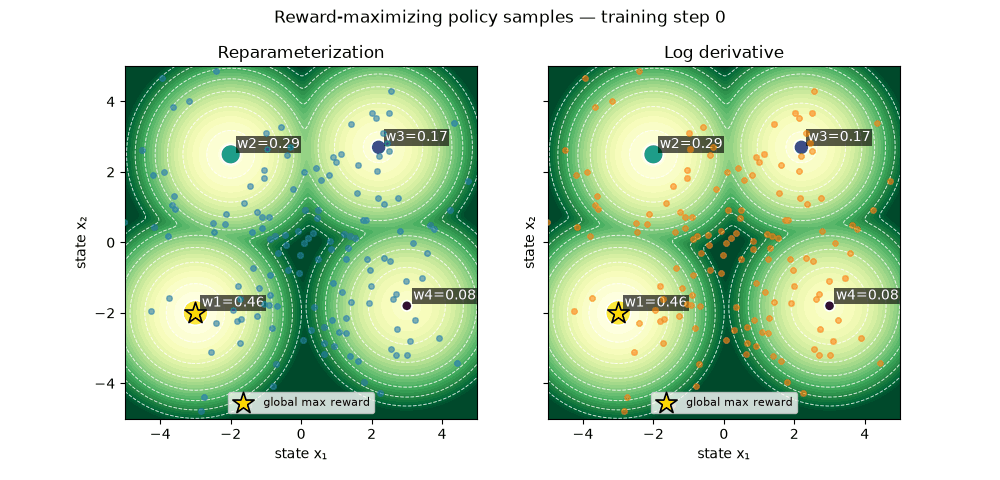
\includegraphics[width=0.92\linewidth]{assets/l1_start.png}}
  \end{columns}
\end{frame}

\begin{frame}[fragile]{Lesson 1 exercise: starter code}
  \centering
  \uncover<1->{%
    \href{run:../L1-VariationalInference/gaussian_policy_student.ipynb}
      {\textcolor{BrandBlue}{\texttt{L1-VariationalInference/gaussian\_policy\_student.ipynb}}}
  }
  \vspace{0.20cm}

  \begin{columns}[T,onlytextwidth]
    \column{0.48\textwidth}
      \begin{block}<2->{A. Pathwise VI loss}
\scriptsize
\begin{verbatim}
def reparameterization_maxent_loss(
    policy, num_samples, temperature
):
    # TODO: construct q_theta
    # TODO: draw with rsample
    # TODO: combine reward and entropy
    raise NotImplementedError(...)
\end{verbatim}
      \end{block}
    \column{0.48\textwidth}
      \begin{block}<3->{B. Log-derivative VI loss}
\scriptsize
\begin{verbatim}
def log_derivative_maxent_loss(
    policy, num_samples, temperature
):
    # TODO: sample and log_prob
    # TODO: reward - temperature*log_prob
    # TODO: detached centered score loss
    raise NotImplementedError(...)
\end{verbatim}
      \end{block}
  \end{columns}
\end{frame}

\begin{frame}[fragile]{Lesson 1 exercise: solution}
  \centering
  \uncover<1->{%
    \href{run:../L1-VariationalInference/gaussian_policy_solution.ipynb}
      {\textcolor{BrandBlue}{\texttt{L1-VariationalInference/gaussian\_policy\_solution.ipynb}}}
  }
  \vspace{0.12cm}

  \begin{columns}[T,onlytextwidth]
    \column{0.48\textwidth}
      \begin{block}<2->{A. Pathwise VI loss}
\scriptsize
\begin{verbatim}
q = policy.distribution()
x = q.rsample((num_samples,))
mean_reward = target_reward(x).mean()
entropy = q.entropy()
return -mean_reward - temperature * entropy
\end{verbatim}
      \end{block}
    \column{0.48\textwidth}
      \begin{block}<3->{B. Log-derivative VI loss}
\scriptsize
\begin{verbatim}
q = policy.distribution()
x = q.sample((num_samples,))
log_q = q.log_prob(x)
signal = target_reward(x) - temperature*log_q
baseline = (signal.sum() - signal)/(num_samples-1)
centered = (signal - baseline).detach()
return -(centered * log_q).mean()
\end{verbatim}
      \end{block}
  \end{columns}
\end{frame}

\begin{frame}{Lesson 1 result: VI balances reward and entropy}
  \centering
  \animategraphics[autoplay,loop,poster=first,width=0.96\linewidth]
    {2}{assets/l2_training/frame-}{0}{40}
  \vspace{0.05cm}

  {\scriptsize At $\Tau=0.5$, both estimators move toward high reward while
  retaining finite variance. The dashed line marks the current optimization step.}
\end{frame}

\section{Lesson 2: Diffusion samplers}

\begin{frame}[plain]
  \begin{tikzpicture}[remember picture,overlay]
    \fill[Navy] (current page.south west) rectangle (current page.north east);
    \fill[Sky] (current page.south west) rectangle
      ([xshift=1.3cm]current page.north west);
    \node[anchor=center,text=white,align=center]
      at ([xshift=0.65cm]current page.center)
      {{\bfseries\fontsize{16}{18}\selectfont LESSON 2}\\[0.24cm]
       {\bfseries\fontsize{25}{28}\selectfont Diffusion Samplers}};
  \end{tikzpicture}
  \plainlogos
\end{frame}

\begin{frame}{Problem statement: make the variational family multimodal}
  \small
  \begin{columns}[T,onlytextwidth]
    \column{0.47\textwidth}
      \begin{block}<1->{The limitation}
        $p_{\Tau}(x)$ may have separated modes; a Gaussian $q_\theta(x)$ has one.
      \end{block}
      \begin{block}<2->{Diffusion variational distribution}
        \[
          \begin{gathered}
            X^K\sim\Normal(0,\nu^2I),\qquad \nu>0,\\[-0.02cm]
            X^K\longrightarrow\cdots\longrightarrow X^0\sim q_\theta.
          \end{gathered}
        \]
        Simple transitions compose into a multimodal endpoint.
      \end{block}
    \column{0.49\textwidth}
      \centering
      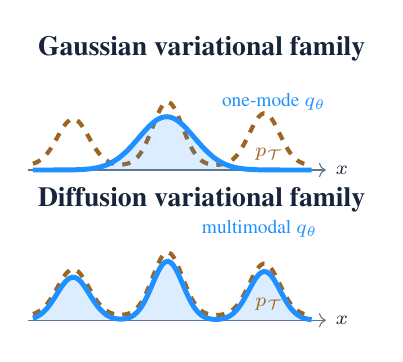
\begin{tikzpicture}[x=0.60cm,y=0.72cm,font=\scriptsize]
        \uncover<1->{%
          \node[anchor=west,font=\bfseries,text=Ink] at (0.25,4.48)
            {Gaussian variational family};
          \draw[->,Slate] (0.25,2.35) -- (6.55,2.35) node[right,text=Ink] {$x$};
          \draw[TrailDark,line width=1.5pt,dashed,domain=0.35:6.25,
                samples=100,smooth]
            plot (\x,{2.43
              +0.82*exp(-4.5*(\x-1.20)^2)
              +1.12*exp(-5.0*(\x-3.20)^2)
              +0.92*exp(-4.8*(\x-5.25)^2)});
          \path[fill=BrandBlue,fill opacity=0.16]
            (0.35,2.35) -- plot[domain=0.35:6.25,samples=90,smooth]
            (\x,{2.35+0.94*exp(-1.45*(\x-3.18)^2)}) -- (6.25,2.35) -- cycle;
          \draw[BrandBlue,line width=1.8pt,domain=0.35:6.25,samples=90,smooth]
            plot (\x,{2.35+0.94*exp(-1.45*(\x-3.18)^2)});
          \node[text=BrandBlue] at (5.45,3.55) {one-mode $q_\theta$};
          \node[text=TrailDark] at (5.35,2.62) {$p_{\Tau}$};
        }

        \uncover<2->{%
          \node[anchor=west,font=\bfseries,text=Ink] at (0.25,1.82)
            {Diffusion variational family};
          \draw[->,Slate] (0.25,-0.30) -- (6.55,-0.30) node[right,text=Ink] {$x$};
          \draw[TrailDark,line width=1.5pt,dashed,domain=0.35:6.25,
                samples=100,smooth]
            plot (\x,{-0.22
              +0.82*exp(-4.5*(\x-1.20)^2)
              +1.12*exp(-5.0*(\x-3.20)^2)
              +0.92*exp(-4.8*(\x-5.25)^2)});
          \path[fill=BrandBlue,fill opacity=0.16]
            (0.35,-0.30) -- plot[domain=0.35:6.25,samples=100,smooth]
            (\x,{-0.30
              +0.76*exp(-4.2*(\x-1.20)^2)
              +1.04*exp(-4.8*(\x-3.20)^2)
              +0.86*exp(-4.5*(\x-5.25)^2)}) -- (6.25,-0.30) -- cycle;
          \draw[BrandBlue,line width=1.8pt,domain=0.35:6.25,
                samples=100,smooth]
            plot (\x,{-0.30
              +0.76*exp(-4.2*(\x-1.20)^2)
              +1.04*exp(-4.8*(\x-3.20)^2)
              +0.86*exp(-4.5*(\x-5.25)^2)});
          \node[text=BrandBlue] at (5.15,1.32) {multimodal $q_\theta$};
          \node[text=TrailDark] at (5.35,-0.02) {$p_{\Tau}$};
        }
      \end{tikzpicture}
  \end{columns}
\end{frame}

\begin{frame}{Diffusion models: variance-preserving noising in discrete time}
  \footnotesize
  \setlength{\abovedisplayskip}{4pt}
  \setlength{\belowdisplayskip}{4pt}
  \begin{columns}[c,onlytextwidth]
    \column{0.51\textwidth}
      \begin{itemize}
        \setlength{\itemsep}{0.20cm}
        \item<1-> \textbf{Start with data} $X^0\sim p_0$; choose small noise steps:
          \[
            \delta_k=\beta_k\Delta_k>0,
            \qquad \textcolor{Slate}{\varepsilon_k}\overset{\mathrm{iid}}{\sim}\Normal(0,1).
          \]
        \item<2-> \textbf{Shrink the signal and add Gaussian noise:}
          \[
            \begin{aligned}
              X^k&=\underbrace{(1-\tfrac12\delta_{k-1})X^{k-1}}_{\text{shrink}}\\
                 &\quad+\underbrace{\textcolor{Slate}{\nu\sqrt{\delta_{k-1}}\,\varepsilon_{k-1}}}_{\text{add noise}}.
            \end{aligned}
          \]
        \item<3-> \textbf{Enough small steps give a Gaussian prior:}
          \[
            \textcolor{TrailDark}{p_K}\approx \textcolor{Slate}{q_K}=\Normal(0,\nu^2).
          \]
          Near the prior, shrinkage balances noise;
          $\nu$ sets its standard deviation.
      \end{itemize}
    \column{0.47\textwidth}
      \centering
      \animategraphics[autoplay,loop,poster=first,width=\linewidth]
        {10}{assets/vp_diffusion_1d/frame-}{0}{79}
      \begin{itemize}
        \item \scriptsize $\nu=1$, $\delta_k=0.02$, $K=600$.
      \end{itemize}
  \end{columns}
  \vfill
  {\tiny\color{Slate}
    The discrete update preserves the prior approximately for small steps.}
\end{frame}

\begin{frame}{Reverse diffusion: from optimal to learned score}
  \footnotesize
  \setlength{\abovedisplayskip}{4pt}
  \setlength{\belowdisplayskip}{4pt}
  \begin{itemize}[<+->]
    \setlength{\itemsep}{0.20cm}
    \item \textbf{Reverse step with the optimal score}
      $\textcolor{TrailDark}{s_k^*(x)}=\partial_x\log p_k(x)$:
      \[
        X^{k-1}=(1+\tfrac12\delta_k)X^k
          +\nu^2\delta_k\,\textcolor{TrailDark}{s_k^*(X^k)}
          +\nu\sqrt{\delta_k}\,\textcolor{Slate}{\varepsilon_k},
        \qquad\textcolor{Slate}{\varepsilon_k}\sim\Normal(0,1).
      \]
    \item \textbf{The optimal score is intractable in general:}
      approximate it with a neural network,
      \[
        \textcolor{BrandBlue}{u_{\Psi}(x,k)}\approx \textcolor{TrailDark}{s_k^*(x)}.
      \]
    \item \textbf{Plug in the learned score:}
      \[
        \boxed{X^{k-1}=(1+\tfrac12\delta_k)X^k
          +\nu^2\delta_k\,{\color{BrandBlue}u_{\Psi}(X^k,k)}
          +\nu\sqrt{\delta_k}\,\textcolor{Slate}{\varepsilon_k}.}
      \]
    \item \textbf{Generate from the Gaussian prior:}
      \[
        \underbrace{X^K\sim\Normal(0,\nu^2)}_{\text{Gaussian prior}}
        \xrightarrow{\textcolor{BrandBlue}{q_\theta}}\;X^{K-1}
        \xrightarrow{\textcolor{BrandBlue}{q_\theta}}\;\cdots
        \xrightarrow{\textcolor{BrandBlue}{q_\theta}}\;
        \underbrace{X^0\sim q_\theta}_{\text{generated sample}}.
      \]
  \end{itemize}
\end{frame}

\begin{frame}{From diffusion models to diffusion samplers}
  \small
  \setlength{\abovedisplayskip}{4pt}
  \setlength{\belowdisplayskip}{4pt}
  \begin{itemize}[<+->]
    \setlength{\itemsep}{0.24cm}
    \item \textbf{Diffusion models:} learn from samples of the target distribution.
    \item \textbf{Our diffusion sampler:} only the cost $\textcolor{TrailDark}{C(x)}$ is available.
      \[
        \textcolor{TrailDark}{p_{\Tau}}(x)=\frac{e^{-\textcolor{TrailDark}{C(x)}/\Tau}}{Z_{\Tau}},
        \qquad \min_\theta\KL\!\left(\textcolor{BrandBlue}{q_\theta}(x^0)\|\textcolor{TrailDark}{p_{\Tau}}(x^0)\right).
      \]
    \item \textbf{Also learnable:} the prior $q_{\phi,K}$ and diffusion
      coefficients $\beta_{0:K}$.\\
      {\footnotesize Exercise: optional coefficient learning; fixed Gaussian prior.}
    \item \textbf{The obstacle:} the marginal distribution
      $\textcolor{BrandBlue}{q_\theta}(x^0)$ is intractable to evaluate.
      \[
        \underbrace{\textcolor{BrandBlue}{q_\theta}(x^0)}_{\text{marginal}}
        =\int\underbrace{\textcolor{BrandBlue}{q_\theta}(x^0,\textcolor{DiffusionLatent}{z})}_{\text{joint}}\,d\textcolor{DiffusionLatent}{z}.
      \]
      Keep the latent variable $Z$ to work with a tractable joint distribution.
  \end{itemize}
\end{frame}

\begin{frame}{Data-processing inequality: introduce a latent variable $Z$}
  \small
  \setlength{\abovedisplayskip}{4pt}
  \setlength{\belowdisplayskip}{4pt}
  \begin{itemize}[<+->]
    \setlength{\itemsep}{0.20cm}
    \item \textbf{Joint distributions over $(X,Z)$ give marginals over $X$:}
      \[
        \textcolor{BrandBlue}{q}(x)=\int q(x,\textcolor{DiffusionLatent}{z})\,d\textcolor{DiffusionLatent}{z},
        \qquad \textcolor{TrailDark}{p}(x)=\int p(x,\textcolor{DiffusionLatent}{z})\,d\textcolor{DiffusionLatent}{z}.
      \]
    \item \textbf{KL chain rule:}
      \[
        \begin{aligned}
          \KL(q(x,\textcolor{DiffusionLatent}{z})\|p(x,\textcolor{DiffusionLatent}{z}))
          &=\KL(q(x)\|p(x))\\
          &\quad+\underbrace{\E_{X\sim q}\!\left[
            \KL(q(\textcolor{DiffusionLatent}{z}\mid X)\|p(\textcolor{DiffusionLatent}{z}\mid X))\right]}_{\geq 0}.
        \end{aligned}
      \]
    \item \textbf{DPI: discarding $Z$ cannot increase KL.}
      \[
        \boxed{\KL(q(x)\|p(x))\leq\KL(q(x,\textcolor{DiffusionLatent}{z})\|p(x,\textcolor{DiffusionLatent}{z})).}
      \]
  \end{itemize}
\end{frame}

\begin{frame}{Apply the DPI to a diffusion path}
  \footnotesize
  \setlength{\abovedisplayskip}{4pt}
  \setlength{\belowdisplayskip}{4pt}
  \begin{itemize}[<+->]
    \setlength{\itemsep}{0.20cm}
    \item \textbf{Substitute $X=X^0$ and $\textcolor{DiffusionLatent}{Z=X^{1:K}}$:}
      \[
        \boxed{\KL(\textcolor{BrandBlue}{q_\theta}(x^0)\|\textcolor{TrailDark}{p_{\Tau}}(x^0))
        \leq \KL(\textcolor{BrandBlue}{q_\theta}(x^{0:K})\|\textcolor{TrailDark}{p_{\Tau}}(x^{0:K}))}
      \]
    \item \textbf{The joint distributions are the full paths:}
      \[
        \begin{aligned}
          \textcolor{BrandBlue}{q_\theta}(x^{0:K})
            &=\textcolor{Slate}{q_K(x^K)}\prod_{k=1}^{K}\textcolor{BrandBlue}{q_\theta}(x^{k-1}\mid x^k),\\
          \textcolor{TrailDark}{p_{\Tau}}(x^{0:K})
            &=\textcolor{TrailDark}{p_{\Tau}}(x^0)\prod_{k=1}^{K}\textcolor{TrailDark}{p}(x^k\mid x^{k-1}).
        \end{aligned}
      \]
    \item \textbf{Trainable loss, up to $\Tau\log Z_{\Tau}$:}
      \[
        L_{\mathrm{path}}
        =\E_{q_\theta}\!\left[
        -\textcolor{TrailDark}{R(x^0)}+\Tau\log \textcolor{Slate}{q_K(x^K)}
        +\Tau\sum_{k=1}^{K}\log
        \frac{\textcolor{BrandBlue}{q_\theta}(x^{k-1}\mid x^k)}
             {\textcolor{TrailDark}{p}(x^k\mid x^{k-1})}\right]
      \]
  \end{itemize}
\end{frame}

\begin{frame}{Optional Langevin preconditioning}
  \begin{itemize}[<+->]
    \item \textbf{Use the target gradient:}
      \[
        \textcolor{TrailDark}{\nabla_x\log p_{\Tau}(x)}
        =-\frac{\textcolor{TrailDark}{\nabla_x C(x)}}{\Tau}
        =\frac{\textcolor{TrailDark}{\nabla_x R(x)}}{\Tau}.
      \]
    \item \textbf{Parameterize the score:}
      \[
        \boxed{\textcolor{BrandBlue}{u_\Psi(x,k)}=-\frac{x}{\nu^2}
          +\mathrm{NN}_1(k,x)
          +\mathrm{NN}_2(k)\odot\textcolor{TrailDark}{\nabla_x\log p_{\Tau}(x)}.}
      \]
  \end{itemize}
\end{frame}

\begin{frame}[fragile]{Lesson 2 exercise: starter code}
  \centering
  \uncover<1->{%
    \href{run:../L2-DiffusionSamplers/diffusion_sampler_student.ipynb}
      {\scriptsize\textcolor{BrandBlue}{\texttt{L2-DiffusionSamplers/diffusion\_sampler\_student.ipynb}}}
  }
  \vspace{-0.22cm}

  \begin{columns}[T,onlytextwidth]
    \column{0.49\textwidth}
      \begin{block}<2->{\small A. Forward: two peaks $\to$ Gaussian}
\fontsize{6.1}{6.8}\selectfont
\begin{verbatim}
def forward_sde_step(previous_state, delta, *,
    reparameterize, noise=None, prior_std=PRIOR_STD):
    # TODO: mean, std, sample; delta = delta_{k-1}
    raise NotImplementedError(...)
# Also implement: forward_kernel_log_prob
\end{verbatim}
      \end{block}
    \column{0.49\textwidth}
      \begin{block}<3->{\small B. Reverse: Gaussian $\to$ two peaks}
\fontsize{6.1}{6.8}\selectfont
\begin{verbatim}
def reverse_sde_step(score_network, noisy_state,
    step_index, delta, num_steps, *, reparameterize,
    noise=None, prior_std=PRIOR_STD):
    # TODO: score, mean, std, sample; delta = delta_k
    raise NotImplementedError(...)
# Also implement: reverse_kernel_log_prob
\end{verbatim}
      \end{block}
  \end{columns}
  \vspace{-0.10cm}
  \uncover<3->{%
    \begin{minipage}{0.90\linewidth}
      \centering
      % Generated by scripts/generate_kernel_preview.py
\animategraphics[autoplay,loop,poster=first,width=\linewidth]{10}{assets/kernel_preview/frame-}{0}{79}

      \par
    \end{minipage}
    \par\vspace{0.02cm}
    \begin{itemize}
      \item \scriptsize $\Normal(0,1)$ prior; $K=600$; linear $\delta_k:0.005\to0.035$.
        Reverse: pretrained score, fixed settings.
    \end{itemize}
  }
\end{frame}

\begin{frame}[fragile]{Lesson 2 exercise: solution}
  \centering
  \uncover<1->{%
    \href{run:../L2-DiffusionSamplers/diffusion_sampler_solution.ipynb}
      {\textcolor{BrandBlue}{\texttt{L2-DiffusionSamplers/diffusion\_sampler\_solution.ipynb}}}
  }
  \vspace{0.06cm}

  \begin{columns}[T,onlytextwidth]
    \column{0.49\textwidth}
      \begin{block}<2->{A. Forward kernel solution}
\fontsize{6.2}{7.0}\selectfont
\begin{verbatim}
# delta = delta_{k-1}
mean = (1.0 - 0.5 * delta) * previous_state
sigma = prior_std * delta.sqrt()
epsilon = torch.randn_like(mean)
sample = mean + sigma * epsilon
if not reparameterize:
    sample = sample.detach()  # stop gradient
return sample

# forward_kernel_log_prob: same mean and sigma
p = Independent(Normal(mean, sigma), 1)
return p.log_prob(noisy_state)
\end{verbatim}
      \end{block}
    \column{0.49\textwidth}
      \begin{block}<3->{B. Reverse kernel solution}
\fontsize{6.2}{7.0}\selectfont
\begin{verbatim}
# step_index = k; delta = delta_k
score = score_network(noisy_state,
                      step_index, num_steps)
mean = (1.0 + 0.5 * delta) * noisy_state
mean = mean + delta * prior_std**2 * score
sigma = prior_std * delta.sqrt()
epsilon = torch.randn_like(mean)
sample = mean + sigma * epsilon
if not reparameterize:
    sample = sample.detach()  # stop gradient
return sample

# reverse_kernel_log_prob: same mean and sigma
q = Independent(Normal(mean, sigma), 1)
return q.log_prob(previous_state)
\end{verbatim}
      \end{block}
  \end{columns}
\end{frame}

\begin{frame}{GMM-40: reparameterization vs. log derivative}
  \centering
  % Generated by scripts/generate_diffusion_estimator_comparison.py
\animategraphics[autoplay,loop,poster=last,height=0.68\textheight]
  {4}{assets/l4_training/frame-}{0}{76}

  \vspace{0.04cm}

  {\scriptsize
    \begin{itemize}
      \item Fixed $\Tau=1$; 26,000 updates; same seed and noise;
        shared learning-rate decrease after update 20,000.
      \item Without Langevin: log derivative reaches lower loss.
        With Langevin: similar final losses (one seed).
    \end{itemize}}
\end{frame}

\section{Lesson 3: Reinforcement learning as variational inference}

\begin{frame}[plain]
  \begin{tikzpicture}[remember picture,overlay]
    \fill[Navy] (current page.south west) rectangle (current page.north east);
    \fill[Sky] (current page.south west) rectangle
      ([xshift=1.3cm]current page.north west);
    \node[anchor=center,text=white,align=center]
      at ([xshift=0.65cm]current page.center)
      {{\bfseries\fontsize{16}{18}\selectfont LESSON 3}\\[0.24cm]
       {\bfseries\fontsize{24}{27}\selectfont RL as Variational Inference}};
  \end{tikzpicture}
  \plainlogos
\end{frame}

\begin{frame}{The target: high-return trajectories}
  \footnotesize
  \setlength{\abovedisplayskip}{5pt}
  \setlength{\belowdisplayskip}{5pt}
  \begin{columns}[c,onlytextwidth]
    \column{0.43\textwidth}
      \begin{itemize}
        \setlength{\itemsep}{0.23cm}
        \item \textbf{Reward-weighted trajectory target:}
          \[
            \begin{aligned}
              \textcolor{TrailDark}{\pi}(\tau)&=\frac{p(s_0)}{\mathcal Z}
                e^{\textcolor{TrailDark}{G(\tau)}/\Tau}\\
                &\quad\cdot\prod_{t=0}^{T}
                  \textcolor{Slate}{p(s_{t+1}\mid s_t,a_t)},
            \end{aligned}
          \]
          \[
            \textcolor{TrailDark}{G(\tau)}
              =\sum_{t=0}^{T}\textcolor{TrailDark}{R_{\mathrm{env}}(s_t,a_t)}.
          \]
        \item \textbf{Intractable action marginal:}
          \[
            \boxed{\textcolor{TrailDark}{\pi}(a_{0:T})
              =\int\textcolor{TrailDark}{\pi}(\tau)\,ds_{0:T+1}.}
          \]
          Integrate over all possible state trajectories.
      \end{itemize}
    \column{0.55\textwidth}
      \centering
      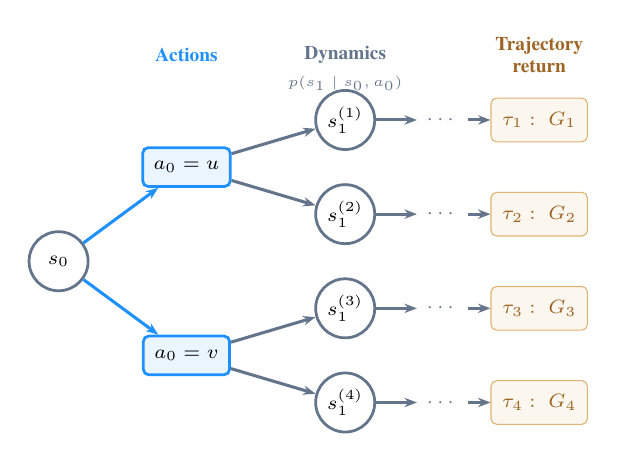
\begin{tikzpicture}[x=1.12cm,y=0.92cm,font=\scriptsize,
          state/.style={circle,draw=Slate,fill=white,line width=1pt,
                        minimum size=7.5mm,inner sep=1pt},
          action/.style={rounded corners=2pt,draw=BrandBlue,fill=BrandBlue!9,
                         line width=1pt,inner xsep=4pt,inner ysep=5pt},
          flow/.style={-{Stealth[length=4.5pt]},line width=1.1pt},
          return/.style={rounded corners=2pt,draw=Trail!75,fill=Trail!9,
                         text=TrailDark,inner xsep=4pt,inner ysep=5pt}]
        % Blue edges enumerate candidate actions, not target-policy probabilities.
        \node[text=BrandBlue,font=\bfseries\scriptsize] at (1.55,2.85) {Actions};
        \node[text=Slate,font=\bfseries\scriptsize] at (3.35,2.85) {Dynamics};
        \node[text=Slate,font=\tiny] at (3.35,2.46)
          {$p(s_1\mid s_0,a_0)$};
        \node[text=TrailDark,font=\bfseries\scriptsize,align=center]
          at (5.55,2.85) {Trajectory\\return};
        \node[state] (root) at (0.10,0) {$s_0$};
        \node[action] (choiceA) at (1.55,1.30) {$a_0=u$};
        \node[action] (choiceB) at (1.55,-1.30) {$a_0=v$};
        \draw[flow,BrandBlue] (root) -- (choiceA);
        \draw[flow,BrandBlue] (root) -- (choiceB);
        \foreach \i/\y/\choice in {1/1.95/A,2/0.65/A,3/-0.65/B,4/-1.95/B}{%
          \node[state] (outcome\i) at (3.35,\y) {$s_1^{(\i)}$};
          % A fixed executed action still branches through stochastic dynamics.
          \draw[flow,Slate] (choice\choice) -- (outcome\i);
          \node[text=Slate] (future\i) at (4.45,\y) {$\cdots$};
          \node[return] (return\i) at (5.55,\y) {$\tau_{\i}:\;G_{\i}$};
          \draw[flow,Slate] (outcome\i) -- (future\i);
          \draw[flow,Slate] (future\i) -- (return\i);
        }
      \end{tikzpicture}
      \vspace{0.08cm}
      \begin{itemize}
        \item \textbf{Same action} $\to$ different future states and returns.
      \end{itemize}
  \end{columns}
\end{frame}

\begin{frame}{A policy induces a distribution over trajectories}
  \footnotesize
  \setlength{\abovedisplayskip}{4pt}
  \setlength{\belowdisplayskip}{4pt}
  \centering
  \textbf{Trajectory: state--action pairs and final state}
  \[
    \tau=\big((s_0,a_0),(s_1,a_1),\ldots,(s_T,a_T),s_{T+1}\big).
  \]
  \vspace{-0.10cm}

  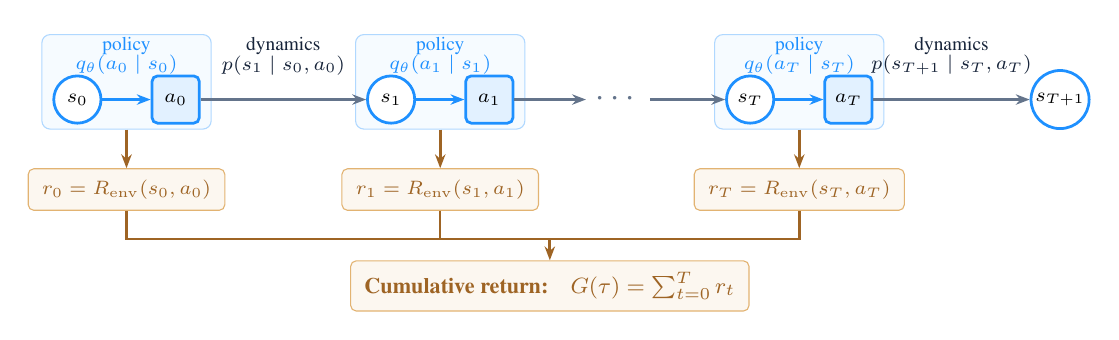
\begin{tikzpicture}[x=0.96cm,y=0.90cm,font=\scriptsize,
      pair/.style={rounded corners=3pt,draw=BrandBlue!35,fill=BrandBlue!4,
                   minimum width=2.15cm,minimum height=1.20cm},
      state/.style={circle,draw=BrandBlue,fill=white,line width=1pt,
                    minimum size=6mm,inner sep=1pt},
      action/.style={rounded corners=2pt,draw=BrandBlue,fill=BrandBlue!13,
                     line width=1pt,minimum size=6mm,inner sep=1pt},
      flow/.style={-{Stealth[length=5pt]},line width=1.15pt},
      reward/.style={rounded corners=2pt,draw=Trail!75,fill=Trail!8,
                     inner xsep=5pt,inner ysep=4pt,align=center,text=TrailDark}]
    \foreach \t/\x in {0/1.10,1/5.25,T/10.00}{%
      \node[pair] (pair\t) at (\x,1.70) {};
      \node[state] (s\t) at ({\x-0.65},1.45) {$s_{\t}$};
      \node[action] (a\t) at ({\x+0.65},1.45) {$a_{\t}$};
      \draw[flow,BrandBlue] (s\t) -- (a\t);
      \node[text=BrandBlue,align=center] at (\x,2.07)
        {policy\\[-1pt] $q_\theta(a_{\t}\mid s_{\t})$};
    }
    \node[state] (terminal) at (13.45,1.45) {$s_{T+1}$};
    \draw[flow,Slate] (a0) -- (s1)
      node[midway,above=5pt,align=center,text=Ink]
        {dynamics\\[-1pt] $p(s_1\mid s_0,a_0)$};
    \node[text=Slate,font=\large] (dots) at (7.60,1.45) {$\cdots$};
    \draw[flow,Slate] (a1) -- (dots);
    \draw[flow,Slate] (dots) -- (sT);
    \draw[flow,Slate] (aT) -- (terminal)
      node[midway,above=5pt,align=center,text=Ink]
        {dynamics\\[-1pt] $p(s_{T+1}\mid s_T,a_T)$};

    \foreach \t/\x in {0/1.10,1/5.25,T/10.00}{%
      \node[reward] (r\t) at (\x,0.18)
        {$r_{\t}=R_{\mathrm{env}}(s_{\t},a_{\t})$};
      \draw[flow,TrailDark] (pair\t.south) -- (r\t.north);
    }
    \node[reward,font=\footnotesize] (return) at (6.70,-1.18)
      {\textbf{Cumulative return:}\quad
       $G(\tau)=\sum_{t=0}^{T}r_t$};
    \draw[TrailDark,line width=0.9pt]
      (r0.south) -- (1.10,-0.52) -- (10.00,-0.52) -- (rT.south);
    \draw[TrailDark,line width=0.9pt] (r1.south) -- (5.25,-0.52);
    \draw[flow,TrailDark] (6.70,-0.52) -- (return.north);
  \end{tikzpicture}
  \vspace{0.08cm}

  \textbf{Expected return:} $\E_{q_\theta}[G(\tau)]$.
\end{frame}

\begin{frame}{From trajectories to variational inference}
  \small
  \setlength{\abovedisplayskip}{5pt}
  \setlength{\belowdisplayskip}{5pt}
  \begin{itemize}[<+->]
    \setlength{\itemsep}{0.18cm}
    \item \textbf{Policy-induced density:} initial density $p(s_0)$.
      \[
        \textcolor{BrandBlue}{q_\theta}(\tau)=p(s_0)\prod_{t=0}^{T}
        \textcolor{BrandBlue}{q_\theta(a_t\mid s_t)}\,
        \textcolor{Slate}{p(s_{t+1}\mid s_t,a_t)}.
      \]
    \item \textbf{Reward-defined target:} temperature $\Tau>0$.
      \[
        \textcolor{TrailDark}{\pi}(\tau):=\frac{1}{\mathcal Z}\,p(s_0)\prod_{t=0}^{T}
        \textcolor{Slate}{p(s_{t+1}\mid s_t,a_t)}\,
        \exp\!\left(\textcolor{TrailDark}{R_{\mathrm{env}}(s_t,a_t)}/\Tau\right).
      \]
    \item \textbf{Action marginals and VI objective:}
      \[
        \begin{aligned}
          \textcolor{BrandBlue}{q_\theta}(a_{0:T})
          &=\int \textcolor{BrandBlue}{q_\theta}(a_{0:T},s_{0:T+1})\,ds_{0:T+1},\\[0.04cm]
          \textcolor{TrailDark}{\pi}(a_{0:T})
          &=\int\textcolor{TrailDark}{\pi}(a_{0:T},s_{0:T+1})\,ds_{0:T+1}.
        \end{aligned}
      \]
      \[
        \boxed{\min_\theta\;\KL\!\left(
          \textcolor{BrandBlue}{q_\theta}(a_{0:T})\|\textcolor{TrailDark}{\pi}(a_{0:T})\right).}
      \]
  \end{itemize}
\end{frame}

\begin{frame}{DPI and reverse KL: maximum-entropy RL}
  \small
  \setlength{\abovedisplayskip}{4pt}
  \setlength{\belowdisplayskip}{4pt}
  \begin{itemize}
    \setlength{\itemsep}{0.18cm}
    \item \textbf{DPI and joint-KL expansion:}
      \[
        \begin{aligned}
          \Tau\KL\!\left(\textcolor{BrandBlue}{q_\theta}(a_{0:T})\|\textcolor{TrailDark}{\pi}(a_{0:T})\right)
          &\leq\Tau\KL\!\left(\textcolor{BrandBlue}{q_\theta}(\tau)\|\textcolor{TrailDark}{\pi}(\tau)\right)\\[0.08cm]
          &=\E_{q_\theta}\!\left[\sum_{t=0}^{T}
            \big(\textcolor{BrandBlue}{\Tau\log q_\theta(a_t\mid s_t)}
            -\textcolor{TrailDark}{R_{\mathrm{env}}(s_t,a_t)}\big)\right]
            +\textcolor{Slate}{\Tau\log\mathcal Z}\\[0.08cm]
          &=-\mathcal J_T(\theta)+\textcolor{Slate}{\Tau\log\mathcal Z}.
        \end{aligned}
      \]
    \item \textbf{Minimize the joint KL $\Longleftrightarrow$ maximize $\mathcal J_T$:}
      \[
        \boxed{\mathcal J_T(\theta)
        :=\E_{q_\theta}\!\left[\sum_{t=0}^{T}
          \big(\textcolor{TrailDark}{R_{\mathrm{env}}(s_t,a_t)}
          -\textcolor{BrandBlue}{\Tau\log q_\theta(a_t\mid s_t)}\big)\right].}
      \]
  \end{itemize}
\end{frame}

\begin{frame}{Maximum-entropy RL: trajectories with soft rewards}
  \footnotesize
  \setlength{\abovedisplayskip}{4pt}
  \setlength{\belowdisplayskip}{4pt}
  \centering
  \textbf{Same trajectories, now with soft rewards}
  \[
    \tau=\big((s_0,a_0),(s_1,a_1),\ldots,(s_T,a_T),s_{T+1}\big).
  \]
  \vspace{-0.10cm}

  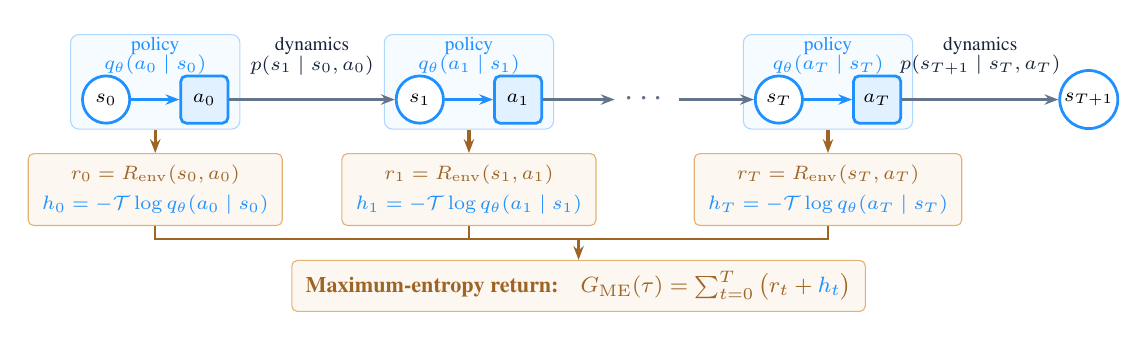
\begin{tikzpicture}[x=0.96cm,y=0.90cm,font=\scriptsize,
      pair/.style={rounded corners=3pt,draw=BrandBlue!35,fill=BrandBlue!4,
                   minimum width=2.15cm,minimum height=1.20cm},
      state/.style={circle,draw=BrandBlue,fill=white,line width=1pt,
                    minimum size=6mm,inner sep=1pt},
      action/.style={rounded corners=2pt,draw=BrandBlue,fill=BrandBlue!13,
                     line width=1pt,minimum size=6mm,inner sep=1pt},
      flow/.style={-{Stealth[length=5pt]},line width=1.15pt},
      reward/.style={rounded corners=2pt,draw=Trail!75,fill=Trail!8,
                     inner xsep=5pt,inner ysep=4pt,align=center,text=TrailDark}]
    \foreach \t/\x in {0/1.10,1/5.25,T/10.00}{%
      \node[pair] (pair\t) at (\x,1.70) {};
      \node[state] (s\t) at ({\x-0.65},1.45) {$s_{\t}$};
      \node[action] (a\t) at ({\x+0.65},1.45) {$a_{\t}$};
      \draw[flow,BrandBlue] (s\t) -- (a\t);
      \node[text=BrandBlue,align=center] at (\x,2.07)
        {policy\\[-1pt] $q_\theta(a_{\t}\mid s_{\t})$};
    }
    \node[state] (terminal) at (13.45,1.45) {$s_{T+1}$};
    \draw[flow,Slate] (a0) -- (s1)
      node[midway,above=5pt,align=center,text=Ink]
        {dynamics\\[-1pt] $p(s_1\mid s_0,a_0)$};
    \node[text=Slate,font=\large] (dots) at (7.60,1.45) {$\cdots$};
    \draw[flow,Slate] (a1) -- (dots);
    \draw[flow,Slate] (dots) -- (sT);
    \draw[flow,Slate] (aT) -- (terminal)
      node[midway,above=5pt,align=center,text=Ink]
        {dynamics\\[-1pt] $p(s_{T+1}\mid s_T,a_T)$};

    \foreach \t/\x in {0/1.10,1/5.25,T/10.00}{%
      \node[reward] (r\t) at (\x,0.18)
        {$r_{\t}=R_{\mathrm{env}}(s_{\t},a_{\t})$\\[3pt]
         \textcolor{BrandBlue}{$h_{\t}=-\Tau\log q_\theta(a_{\t}\mid s_{\t})$}};
      \draw[flow,TrailDark] (pair\t.south) -- (r\t.north);
    }
    \node[reward,font=\footnotesize] (return) at (6.70,-1.18)
      {\textbf{Maximum-entropy return:}\quad
       $G_{\mathrm{ME}}(\tau)=\sum_{t=0}^{T}
         \big(r_t+\textcolor{BrandBlue}{h_t}\big)$};
    \draw[TrailDark,line width=0.9pt]
      (r0.south) -- (1.10,-0.52) -- (10.00,-0.52) -- (rT.south);
    \draw[TrailDark,line width=0.9pt] (r1.south) -- (5.25,-0.52);
    \draw[flow,TrailDark] (6.70,-0.52) -- (return.north);
  \end{tikzpicture}
  \vspace{0.08cm}

  \textcolor{BrandBlue}{\textbf{Entropy bonus:}}
  $\E[\textcolor{BrandBlue}{h_t}\mid s_t]=\textcolor{BrandBlue}{\Tau\,\entropy[q_\theta(\cdot\mid s_t)]}$,
  \qquad $\mathcal J_T(\theta)=\E_{q_\theta}[G_{\mathrm{ME}}(\tau)]$.
\end{frame}

\begin{frame}{Infinite horizon: discount reward and entropy together}
  \footnotesize
  \only<1->{%
    \begin{tikzpicture}[remember picture,overlay]
      \node[anchor=north east,fill=white,rounded corners=1.2pt,
            inner xsep=2.8pt,inner ysep=1.8pt]
        at ([xshift=-0.16cm,yshift=-0.10cm]current page.north east)
        {
\includegraphics[height=0.52cm]{assets/logos/tum_logo.png}};
    \end{tikzpicture}%
  }
  \begin{columns}[T,onlytextwidth]
    \column{0.60\textwidth}
      \begin{block}<1->{Start with a finite cutoff $T$}
        \[
          \mathcal J_T(\theta)
          =\sum_{t=0}^{T}\E_{q_\theta}\!\left[
          \textcolor{TrailDark}{R_t(s_t,a_t)}-\textcolor{BrandBlue}{\Tau_t\log q_\theta(a_t\mid s_t)}\right].
        \]
        \uncover<2->{%
          \textbf{Choose deterministic time weights}
          \[
            \boxed{\textcolor{BrandBlue}{\Tau_t}:=\gamma^t\textcolor{BrandBlue}{\Tau}},\qquad
            \boxed{\textcolor{TrailDark}{R_t(s_t,a_t)}:=\gamma^t\textcolor{TrailDark}{R_{\mathrm{env}}(s_t,a_t)}},
            \quad \gamma\in[0,1).
          \]
        }
      \end{block}
      \uncover<3->{%
        \textbf{Substitute and factor out $\gamma^t$:}
        \[
          \mathcal J_T(\theta)
          =\sum_{t=0}^{T}\gamma^t\E_{q_\theta}\!\left[
          \textcolor{TrailDark}{R_{\mathrm{env}}(s_t,a_t)}-\textcolor{BrandBlue}{\Tau\log q_\theta(a_t\mid s_t)}
          \right].
        \]
      }

    \column{0.36\textwidth}
      \centering
      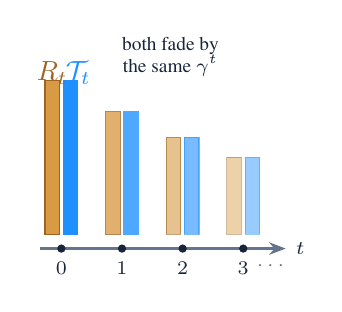
\begin{tikzpicture}[x=0.77cm,y=0.61cm,font=\scriptsize]
        \uncover<1->{%
          \draw[-{Stealth[length=6pt]},Slate,line width=0.9pt]
            (0.30,0.55) -- (4.35,0.55) node[right,text=Ink] {$t$};
          \foreach \x/\lab in {0.65/0,1.65/1,2.65/2,3.65/3}{
            \fill[Ink] (\x,0.55) circle (1.5pt);
            \node[below,text=Ink] at (\x,0.48) {$\lab$};
          }
          \node[below,text=Slate] at (4.13,0.48) {$\cdots$};
        }
        \uncover<2->{%
          \foreach \x/\h/\op in {0.65/3.20/1.00,1.65/2.55/0.78,
                                   2.65/2.02/0.60,3.65/1.60/0.46}{
            \path[fill=Trail,fill opacity=\op,draw=TrailDark,draw opacity=\op]
              ({\x-0.27},0.85) rectangle ({\x-0.03},{0.85+\h});
            \path[fill=BrandBlue,fill opacity=\op,draw=BrandBlue,draw opacity=\op]
              ({\x+0.03},0.85) rectangle ({\x+0.27},{0.85+\h});
          }
          \node[text=TrailDark,font=\bfseries] at (0.50,4.20) {$R_t$};
          \node[text=BrandBlue,font=\bfseries] at (0.93,4.20) {$\Tau_t$};
          \node[text=Ink,align=center] at (2.45,4.55)
            {both fade by\\the same $\gamma^t$};
        }
      \end{tikzpicture}
  \end{columns}
\end{frame}

\begin{frame}{Infinite horizon: now let $T\to\infty$}
  \small
  \begin{itemize}[<+->]
    \item \textbf{Standard maximum-entropy RL objective:}
      \[
        \boxed{
        \mathcal J(\theta)=\E_{q_\theta}\!\left[
        \sum_{t=0}^{\infty}\gamma^t
        \left(\textcolor{TrailDark}{R_{\mathrm{env}}(s_t,a_t)}
        -\textcolor{BrandBlue}{\Tau\log q_\theta(a_t\mid s_t)}\right)
        \right].}
      \]
    \item \textbf{Example: Soft Actor-Critic.}\\
      \href{https://arxiv.org/abs/1801.01290}
        {\textcolor{BrandBlue}{Haarnoja et al. (2018), \emph{Soft Actor-Critic}.}}
    \item \textbf{Reward $+$ policy entropy:} both discounted by $\gamma^t$;
      $\Tau$ controls their trade-off.
  \end{itemize}
\end{frame}

% Local gradient identity: ICLR2027 draft, Sec. 2.1, Eqs. (2)--(3).
\begin{frame}{Maximum-entropy policy gradients: one local actor loss}
  \small
  \setlength{\abovedisplayskip}{4pt}
  \setlength{\belowdisplayskip}{4pt}
  \begin{itemize}
    \setlength{\itemsep}{0.17cm}
    \item \textbf{Policy-gradient theorem $\Rightarrow$ minimize $\mathcal L_{\mathrm{ME}}$:}
      \[
        \mathcal L_{\mathrm{ME}}(\theta)
        :=\frac{1}{1-\gamma}
        \E_{\substack{s\sim d_r\\a\sim q_\theta(\cdot\mid s)}}\!\left[
          \textcolor{BrandBlue}{\Tau\log q_\theta(a\mid s)}-\textcolor{Slate}{Q^{\thetar}}(s,a)\right].
      \]
      Frozen rollout critic $\textcolor{Slate}{Q^{\thetar}}$ and discounted state distribution $d_r$.
    \item \textbf{Soft Bellman equations for $q_{\thetar}$:}
      \[
        \begin{aligned}
          \textcolor{Slate}{Q^{\thetar}}(s,a)&=\textcolor{TrailDark}{R_{\mathrm{env}}(s,a)}
            +\gamma\,\E_{s'\sim p(\cdot\mid s,a)}[\textcolor{Slate}{V^{\thetar}}(s')],\\
          \textcolor{Slate}{V^{\thetar}}(s)&=\E_{a\sim q_{\thetar}(\cdot\mid s)}\!\left[
            \textcolor{Slate}{Q^{\thetar}}(s,a)-\textcolor{BrandBlue}{\Tau\log q_{\thetar}(a\mid s)}\right].
        \end{aligned}
      \]
    \item \textbf{Gradient equivalence at the rollout parameters:}
      \[
        \boxed{\left.\nabla_\theta\mathcal L_{\mathrm{ME}}(\theta)\right|_{\textcolor{Slate}{\theta=\thetar}}
        =-\left.\nabla_\theta\mathcal J(\theta)\right|_{\textcolor{Slate}{\theta=\thetar}}.}
      \]
      Exact at $\theta^{(0)}=\thetar$; later updates use a local approximation.
  \end{itemize}
  \vspace{0.03cm}
  {\scriptsize Exact critic and expectations;
    $d_r(s)=(1-\gamma)\sum_{t\geq0}\gamma^t\Pr_{q_{\thetar}}(s_t=s)$.}
\end{frame}

% TRPO motivates limiting policy changes; a soft KL penalty is one example.
\begin{frame}{Multiple actor updates: a KL penalty}
  \small
  \begin{itemize}
    \setlength{\itemsep}{0.35cm}
    \item \textbf{Several updates on one batch:}
      frozen $d_r$ and $\textcolor{Slate}{Q^{\thetar}}$.
    \item \textbf{TRPO idea:} stay close to the original rollout policy $\textcolor{Slate}{q_{\thetar}}$.
    \item \textbf{For example: an additional KL penalty}
      \[
        \mathcal L_{\mathrm{actor}}(\theta)
        =\mathcal L_{\mathrm{ME}}(\theta)
        +\textcolor{TrailDark}{\lambda_{\mathrm{KL}}}\,
        \E_{s\sim d_r}\!\left[
          \KL\!\left(\textcolor{Slate}{q_{\thetar}}(\cdot\mid s)\|\textcolor{BrandBlue}{q_\theta}(\cdot\mid s)\right)
        \right].
      \]
  \end{itemize}
  \vspace{0.15cm}
  {\scriptsize
    \href{https://arxiv.org/abs/1502.05477}
      {\textcolor{BrandBlue}{Schulman et al. (2015), TRPO.}}}
\end{frame}

\begin{frame}{Example algorithm: REPPO}
  \scriptsize
  \setlength{\abovedisplayskip}{3pt}
  \setlength{\belowdisplayskip}{3pt}
  \begin{columns}[T,onlytextwidth]
    \column{0.56\textwidth}
      \begin{block}{Final REPPO policy loss}
        \[
          \boxed{%
          \mathcal L_{\mathrm{REPPO}}(\theta)
          =\E_{s_i\sim d^{q_{\thetar}}}\!\left[
          \begin{cases}
            \textcolor{BrandBlue}{\mathcal L_{\mathrm{policy}}^{(i)}}(\theta),
              & \widehat D_i\leq\delta_{\mathrm{KL}},\\[0.10cm]
            \textcolor{TrailDark}{\lambda_{\mathrm{KL}}\widehat D_i},
              & \widehat D_i>\delta_{\mathrm{KL}}.
          \end{cases}\right]}
        \]
      \end{block}

      \[
        \begin{gathered}
          \textcolor{BrandBlue}{\mathcal L_{\mathrm{policy}}^{(i)}}
          =-\textcolor{Slate}{Q_\phi(s_i,a_i)}
           +\textcolor{BrandBlue}{\Tau\log q_\theta(a_i\mid s_i)},
          \quad a_i=g_\theta(\varepsilon_i,s_i),\\[0.08cm]
          \widehat D_i
          =\widehat D_{\mathrm{KL}}\!\left(
             \textcolor{Slate}{q_{\thetar}}(\cdot\mid s_i)
             \,\middle\|\,
             \textcolor{BrandBlue}{q_\theta}(\cdot\mid s_i)\right)
          \quad\text{(behavior $\boldsymbol{\to}$ current).}
        \end{gathered}
      \]

    \column{0.41\textwidth}
      \centering
      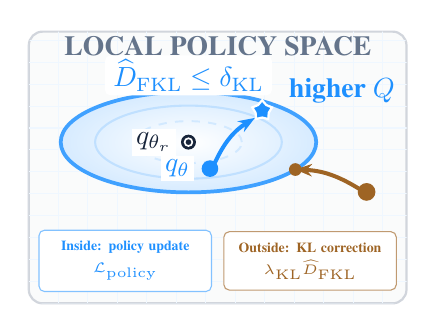
\begin{tikzpicture}[x=0.78cm,y=0.58cm,font=\tiny,
          flow/.style={-{Stealth[length=6pt]},line width=1.45pt},
          legend/.style={fill=white,rounded corners=2pt,
            text width=1.98cm,align=center,inner xsep=3pt,
            inner ysep=4pt,minimum height=0.64cm}]
        \path[fill=Ink!2,draw=Slate!30,rounded corners=5pt,line width=0.8pt]
          (0,0) rectangle (6.15,5.95);
        \begin{scope}
          \clip[rounded corners=5pt] (0,0) rectangle (6.15,5.95);
          \draw[BrandBlue!7,step=0.48] (0,0) grid (6.2,6.0);
        \end{scope}
        \node[text=Slate,font=\bfseries] at (3.08,5.62)
          {LOCAL POLICY SPACE};

        \begin{scope}[shift={(2.60,3.53)}]
            \shade[inner color=white,outer color=BrandBlue!18,
                   draw=BrandBlue!85,line width=1.35pt]
              (0,0) ellipse[x radius=2.08,y radius=1.10];
            \draw[BrandBlue!28,line width=0.75pt]
              (0,0) ellipse[x radius=1.52,y radius=0.80];
            \draw[BrandBlue!20,dashed,line width=0.70pt]
              (0,0) ellipse[x radius=0.87,y radius=0.46];
        \end{scope}
        \node[text=BrandBlue,font=\bfseries,fill=white,rounded corners=2pt,
                inner xsep=3pt,inner ysep=1.6pt]
            at (2.60,4.99) {$\widehat D_{\mathrm{FKL}}\leq\delta_{\mathrm{KL}}$};
        \fill[Ink] (2.60,3.53) circle (2.7pt);
        \draw[white,line width=0.6pt] (2.60,3.53) circle (1.4pt);
        \node[text=Ink,anchor=east,font=\bfseries,
                fill=white,inner sep=1.5pt] at (2.40,3.53)
          {$q_{\thetar}$};

        \node[star,star points=5,fill=BrandBlue,draw=white,
                line width=0.8pt,minimum size=7.5pt,inner sep=0pt]
            (goal) at (3.80,4.22) {};
        \node[text=BrandBlue,anchor=west,font=\bfseries]
          at (4.08,4.66) {higher $Q$};
        \fill[BrandBlue] (2.95,2.95) circle (3.0pt);
        \node[text=BrandBlue,anchor=east,font=\bfseries,
                fill=white,inner sep=1.5pt]
          at (2.70,2.95) {$q_\theta$};
        \draw[flow,BrandBlue] (3.02,3.05) to[bend left=17]
          (goal.south west);

        \fill[TrailDark] (5.50,2.44) circle (3.2pt);
        \draw[flow,TrailDark] (5.40,2.49) to[bend right=15]
          (4.34,2.93);
        \fill[TrailDark] (4.34,2.93) circle (2.3pt);

        % Keep arrow descriptions in separate cards, clear of policy markers.
        \node[legend,draw=BrandBlue!55,text=BrandBlue] at (1.57,0.93)
          {\textbf{Inside: policy update}\\[2pt]
           $\mathcal L_{\mathrm{policy}}$};
        \node[legend,draw=TrailDark!65,text=TrailDark] at (4.58,0.93)
          {\textbf{Outside: KL correction}\\[2pt]
           $\lambda_{\mathrm{KL}}\widehat D_{\mathrm{FKL}}$};
      \end{tikzpicture}
  \end{columns}
  \vspace{0.14cm}

  {\centering
    $\lambda_{\mathrm{KL}}=e^{\omega_{\mathrm{KL}}}$,
    $\Tau=e^{\omega_{\Tau}}$
    \qquad\text{(positive multipliers)}
    \qquad
    \href{https://proceedings.iclr.cc/paper_files/paper/2026/hash/3c2fd72a28fb98facf98546727320249-Abstract-Conference.html}
      {\textcolor{BrandBlue}{Voelcker et al. (2026)}}
    \par}
  \vspace{-0.08cm}

  \begin{columns}[T,onlytextwidth]
    \column{0.49\textwidth}
      \begin{block}{KL-multiplier update}
        \[
          \boxed{%
          \omega_{\mathrm{KL}}^{n+1}
          =\omega_{\mathrm{KL}}^{n}
          +\eta_{\mathrm{KL}}\lambda_{\mathrm{KL}}
          \left(
            \E_s\!\left[\textcolor{TrailDark}{\widehat D_{\mathrm{FKL}}(s)}\right]
            -\delta_{\mathrm{KL}}
          \right)}
        \]
      \end{block}
    \column{0.49\textwidth}
      \begin{block}{Temperature update}
        \[
          \boxed{%
          \omega_{\Tau}^{n+1}
          =\omega_{\Tau}^{n}
          +\eta_{\Tau}\Tau
          \left(
            \textcolor{BrandBlue}{\mathcal H_{\mathrm{tar}}}
            -\E_s\!\left[\textcolor{BrandBlue}{\mathcal H[q_\theta(\cdot\mid s)]}\right]
          \right)}
        \]
      \end{block}
  \end{columns}
\end{frame}

\begin{frame}{Multimodal Agent: benchmark and optimal behavior}
  \small
  \begin{itemize}
    \setlength{\itemsep}{0.06cm}
    \item \textbf{State:} eight headings $0^\circ,45^\circ,\ldots,315^\circ$;
      \textbf{action:} $a\in[-1,1]$.
    \item \textbf{Motion:} turn command $90^\circ a$, snapped to $\pm45^\circ$;
      one forward step.
  \end{itemize}
  \vspace{0.10cm}
  \begin{columns}[T,onlytextwidth]
    \column{0.48\textwidth}
      \centering
      \textbf{Bimodal reward landscape}\par\vspace{0.08cm}
      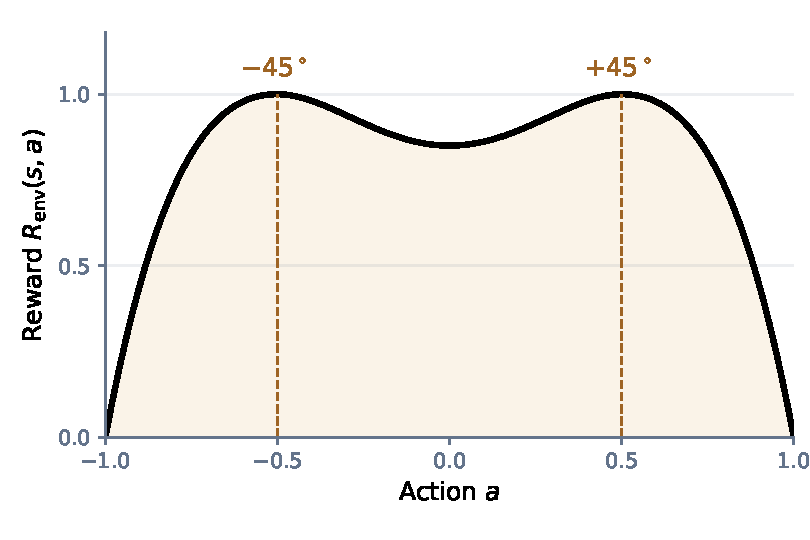
\includegraphics[width=0.94\linewidth]{assets/multimodal_agent_reward.pdf}
      \par\vspace{0.06cm}
      {\scriptsize Same reward for every heading.}
    \column{0.48\textwidth}
      \centering
      \textbf{Reward-optimal behavior}\par\vspace{0.08cm}
      \animategraphics[autoplay,loop,poster=last,width=0.94\linewidth]
        {5}{assets/multimodal_agent_optimal/frame-}{0}{25}
      \par\vspace{0.06cm}
      {\scriptsize Random choice of $a=\pm0.5$ at each step.\\
        Colored lines: independent rollouts.}
  \end{columns}
\end{frame}

\begin{frame}{REPPO on the Multimodal Agent benchmark}
  \small
  \begin{columns}[T,onlytextwidth]
    \column{0.49\textwidth}
      \centering
      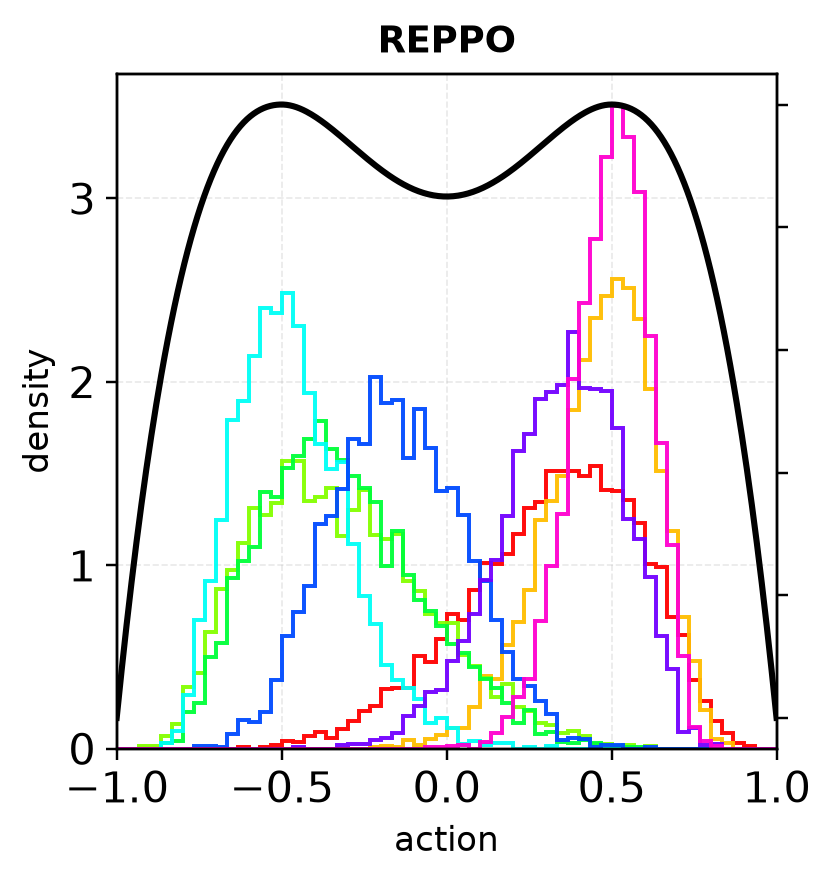
\includegraphics[height=0.61\textheight]
        {assets/multimodal_agent_reppo_histogram.png}

    \column{0.47\textwidth}
      \begin{itemize}[<+->]
        \item \textbf{REPPO:} Gaussian policy $q_\theta(a\mid s)$.
        \item \textbf{Result:} one reward peak per state; second mode missing.
      \end{itemize}
      \vspace{0.20cm}
      \uncover<2->{\scriptsize
        Colored histograms: $q_\theta(a\mid s)$ at the headings below.\quad
        \href{https://arxiv.org/abs/2512.02019}
          {\textcolor{BrandBlue}{Sanokowski \& Patil (2026)}}.}
  \end{columns}
  \vspace{0.10cm}

  {\centering\multimodalstatelegend\par}
\end{frame}

\begin{frame}{REPPO behavior versus the optimal multimodal behavior}
  \centering
  \begin{columns}[onlytextwidth]
    \column{0.49\textwidth}
      \centering\bfseries REPPO: one mode per state
    \column{0.49\textwidth}
      \centering\bfseries Reward-optimal reference
  \end{columns}
  \vspace{0.08cm}

  \animategraphics[autoplay,loop,poster=last,width=0.96\linewidth]
    {5}{assets/multimodal_agent_reppo_vs_optimal/frame-}{0}{25}
  \vspace{0.08cm}

  \small
  \begin{itemize}
    \item \textbf{REPPO:} one diagonal family of trajectories.
    \item \textbf{Optimal reference:} diverse rollouts using both reward-maximizing turns.
  \end{itemize}
\end{frame}

\section{Lesson 4: Diffusion-augmented MDPs}

\begin{frame}[plain]
  \begin{tikzpicture}[remember picture,overlay]
    \fill[Navy] (current page.south west) rectangle (current page.north east);
    \fill[Sky] (current page.south west) rectangle
      ([xshift=1.3cm]current page.north west);
    \node[anchor=center,text=white,align=center]
      at ([xshift=0.65cm]current page.center)
      {{\bfseries\fontsize{16}{18}\selectfont LESSON 4}\\[0.24cm]
       {\bfseries\fontsize{24}{27}\selectfont Diffusion-Augmented MDPs}};
  \end{tikzpicture}
  \plainlogos
\end{frame}

\begin{frame}{RL as variational inference, now with a diffusion policy}
  \footnotesize
  \setlength{\abovedisplayskip}{5pt}
  \setlength{\belowdisplayskip}{5pt}
  \begin{itemize}
    \setlength{\itemsep}{0.20cm}
    \item \textbf{Recall the RL-as-VI objective:} horizon $H$; executed actions $a_t=a_t^0$.
      \[
        \boxed{\min_\theta\;\KL\!\left(
          \textcolor{BrandBlue}{q_\theta}(a_{0:H}^0)
          \,\middle\|\,
          \textcolor{TrailDark}{\pi}(a_{0:H}^0)\right).}
      \]
    \item \textbf{Now use a diffusion model for the policy:}
      \[
        \textcolor{DiffusionLatent}{a_t^K}\sim q_{\mathrm{prior}}
        \;\xrightarrow{\;\textcolor{BrandBlue}{q_\theta}\;}\;
        \textcolor{DiffusionLatent}{a_t^{K-1}}
        \;\longrightarrow\;\cdots\;
        \xrightarrow{\;\textcolor{BrandBlue}{q_\theta}\;}\;a_t^0.
      \]
    \item \textbf{New obstacle: the policy density is a marginal.}
      \[
        \underbrace{\textcolor{BrandBlue}{q_\theta}(a_t^0\mid s_t)}_{
          \text{intractable density}}
        =\int
          \underbrace{q_{\mathrm{prior}}(a_t^K)
            \prod_{k=1}^{K}\textcolor{BrandBlue}{q_\theta}
              (a_t^{k-1}\mid a_t^k,s_t)}_{\text{tractable diffusion-path factors}}
          \,d\textcolor{DiffusionLatent}{a_t^{1:K}}.
      \]
      \begin{itemize}
        \item Cannot directly evaluate $\log q_\theta(a_t^0\mid s_t)$ in the RL loss.
      \end{itemize}
  \end{itemize}
\end{frame}

\begin{frame}{DPI again: keep the diffusion variables}
  \footnotesize
  \setlength{\abovedisplayskip}{5pt}
  \setlength{\belowdisplayskip}{5pt}
  \[
    A=a_{0:H}^0,\qquad \textcolor{Slate}{S=s_{0:H+1}},\qquad
    \textcolor{DiffusionLatent}{Z=a_{0:H}^{1:K}}.
  \]
  \begin{itemize}
    \setlength{\itemsep}{0.20cm}
    \item \textbf{Retain $Z$: marginals become joint diffusion paths.}
      \[
        \begin{aligned}
          \textcolor{BrandBlue}{q_\theta}(A,S)
            &=\int\textcolor{BrandBlue}{q_\theta}
              (A,S,\textcolor{DiffusionLatent}{Z})
                \,d\textcolor{DiffusionLatent}{Z},\\[0.06cm]
          \textcolor{TrailDark}{\pi}(A,S)
            &=\int\textcolor{TrailDark}{\pi_\theta}
              (A,S,\textcolor{DiffusionLatent}{Z})
                \,d\textcolor{DiffusionLatent}{Z}.
        \end{aligned}
      \]
    \item \textbf{Apply the same inequality again:}
      \[
        \begin{aligned}
          \KL\!\left(q_\theta(A)\|\pi(A)\right)
          &\;\underset{\textcolor{Slate}{\text{Lesson 3: retain states}}}{\leq}\;
            \KL\!\left(q_\theta(A,\textcolor{Slate}{S})
              \,\middle\|\,\pi(A,\textcolor{Slate}{S})\right)\\[0.24cm]
          &\;\underset{\textcolor{DiffusionLatent}{\text{Now: retain denoising}}}{\leq}\;
            \boxed{\KL\!\left(
              \textcolor{BrandBlue}{q_\theta}(A,S,\textcolor{DiffusionLatent}{Z})
              \,\middle\|\,
              \textcolor{TrailDark}{\pi_\theta}(A,S,\textcolor{DiffusionLatent}{Z})
            \right).}
        \end{aligned}
      \]
    \item \textbf{Same target marginal:} forward noising adds $Z$;
      $\pi(A,S)$ stays fixed.
  \end{itemize}
\end{frame}

\begin{frame}{Joint diffusion paths: products of tractable kernels}
  \footnotesize
  \setlength{\abovedisplayskip}{6pt}
  \setlength{\belowdisplayskip}{6pt}
  \[
    A=a_{0:H}^0,\qquad S=s_{0:H+1},\qquad
    \textcolor{DiffusionLatent}{Z=a_{0:H}^{1:K}}.
  \]
  \begin{itemize}
    \setlength{\itemsep}{0.25cm}
    \item \textbf{Variational joint: prior + reverse denoising.}
      \[
        \begin{aligned}
          \textcolor{BrandBlue}{q_\theta}(A,S,\textcolor{DiffusionLatent}{Z})
          &=\textcolor{Slate}{p(s_0)
              \prod_{t=0}^{H}p(s_{t+1}\mid s_t,a_t^0)}\\[0.08cm]
          &\quad\cdot\prod_{t=0}^{H}\!\left[
            q_{\mathrm{prior}}(\textcolor{DiffusionLatent}{a_t^K})
            \prod_{k=1}^{K}\textcolor{BrandBlue}{q_\theta(a_t^{k-1}\mid a_t^k,s_t)}
          \right].
        \end{aligned}
      \]
    \item \textbf{Target joint: original trajectory target + forward noising.}
      \[
        \textcolor{TrailDark}{\pi_\theta}(A,S,\textcolor{DiffusionLatent}{Z})
        =\underbrace{\pi(A,S)}_{\text{original target}}
          \prod_{t=0}^{H}\prod_{k=1}^{K}
            \textcolor{TrailDark}{\pi_\theta(a_t^k\mid a_t^{k-1},s_t)}.
      \]
    \item \textbf{Local factors replace the policy marginal}
      $q_\theta(a_t^0\mid s_t)$.
  \end{itemize}
  \vfill
  \centering
  {\scriptsize
    \textcolor{BrandBlue}{Reverse policy $q_\theta$}\quad
    \textcolor{TrailDark}{Forward reference $\pi_\theta$}\quad
    \textcolor{DiffusionLatent}{Added diffusion variables $Z$}}
\end{frame}

\begin{frame}{DA-MDPs: denoising steps become RL decisions}
  \footnotesize
  \setlength{\abovedisplayskip}{4pt}
  \setlength{\belowdisplayskip}{4pt}
  \begin{itemize}
    \item \textbf{Augmented state} $\widetilde s_{t,k}=(s_t,a_t^k,k)$;
      \textbf{local action} $a_t^{k-1}$. Example: $K=3$.
  \end{itemize}
  \centering
  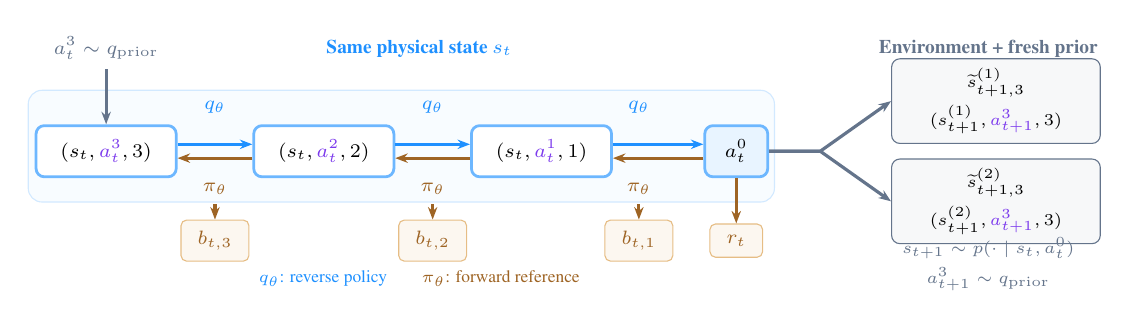
\begin{tikzpicture}[x=0.97cm,y=0.86cm,font=\scriptsize,
      state/.style={rounded corners=3pt,draw=BrandBlue!65,fill=white,
                    line width=1pt,minimum width=1.78cm,minimum height=0.65cm,
                    inner xsep=4pt},
      flow/.style={-{Stealth[length=4.5pt]},line width=1.15pt},
      bonus/.style={rounded corners=2pt,draw=Trail!65,fill=Trail!8,
                    inner xsep=6pt,inner ysep=4pt,text=TrailDark}]
    % One band for the physical state held fixed throughout denoising.
    \path[draw=BrandBlue!20,fill=BrandBlue!3,rounded corners=5pt]
      (0.03,0.45) rectangle (9.80,2.10);
    \node[text=BrandBlue,font=\bfseries\scriptsize] at (5.15,2.72)
      {Same physical state $s_t$};
    \foreach \k/\x in {3/1.05,2/3.90,1/6.75}{%
      \node[state] (state\k) at (\x,1.20)
        {$(s_t,\textcolor{DiffusionLatent}{a_t^\k},\k)$};
    }
    \node[state,minimum width=0.80cm,fill=BrandBlue!10] (execute) at (9.30,1.20)
      {$a_t^0$};
    \node[text=Slate] (prior) at (1.05,2.72)
      {$a_t^3\sim q_{\mathrm{prior}}$};
    \draw[flow,Slate] (prior) -- (state3.north);

    % Blue is the actual policy draw; orange is the forward reference only.
    \foreach \left/\right/\mid/\k in {
        state3/state2/2.475/3,state2/state1/5.325/2,state1/execute/8.025/1}{%
      \draw[flow,BrandBlue]
        ([yshift=2.5pt]\left.east) -- ([yshift=2.5pt]\right.west);
      \node[text=BrandBlue] at (\mid,1.85) {$q_\theta$};
      \draw[flow,TrailDark]
        ([yshift=-2.5pt]\right.west) -- ([yshift=-2.5pt]\left.east);
      \node[text=TrailDark] at (\mid,0.64) {$\pi_\theta$};
      \node[bonus] (bonus\k) at (\mid,-0.12) {$b_{t,\k}$};
      \draw[flow,TrailDark] (\mid,0.42) -- (bonus\k.north);
    }
    \node[bonus] (reward) at (9.30,-0.12) {$r_t$};
    \draw[flow,TrailDark] (execute.south) -- (reward.north);

    % Execute only the final action, branch through physical dynamics, then
    % sample a fresh prior and reset the diffusion phase on each new state.
    \node[text=Slate,font=\bfseries\scriptsize] at (12.60,2.72)
      {Environment + fresh prior};
    \foreach \i/\y in {1/1.94,2/0.46}{%
      \node[draw=Slate,fill=Slate!5,rounded corners=3pt,
            minimum width=2.65cm,minimum height=0.78cm,
            inner xsep=3pt,align=center,font=\fontsize{6.3}{7.2}\selectfont]
        (next\i) at (12.70,\y)
        {$\widetilde s_{t+1,3}^{(\i)}$\\[2pt]
         $(s_{t+1}^{(\i)},\textcolor{DiffusionLatent}{a_{t+1}^3},3)$};
      \draw[flow,Slate] (execute.east) -- (10.40,1.20) -- (next\i.west);
    }
    \node[text=Slate,align=center,font=\fontsize{6.3}{7.2}\selectfont]
      at (12.60,-0.47)
      {$s_{t+1}\sim p(\cdot\mid s_t,a_t^0)$\\[2pt]
       $a_{t+1}^3\sim q_{\mathrm{prior}}$};
    \node[font=\fontsize{6.3}{7.2}\selectfont] at (5.15,-0.68)
      {\textcolor{BrandBlue}{$q_\theta$: reverse policy}\qquad
       \textcolor{TrailDark}{$\pi_\theta$: forward reference}};
  \end{tikzpicture}

  \[
    b_{t,k}=-\Tau\log
      \frac{\textcolor{BrandBlue}{q_\theta(a_t^{k-1}\mid a_t^k,s_t)}}
           {\textcolor{TrailDark}{\pi_\theta(a_t^k\mid a_t^{k-1},s_t)}},
    \qquad r_t=R_{\mathrm{env}}(s_t,a_t^0).
  \]
  \[
    \boxed{\mathcal J_{\mathrm{DA}}(\theta)
      =\E_{q_\theta}\!\left[\sum_{t=0}^{\infty}\gamma^t
        \left(r_t+\sum_{k=1}^{K}b_{t,k}\right)\right].}
  \]
  \begin{itemize}
    \item \scriptsize Joint KL $\to$ discounted return;
      fixed prior, constants omitted.
  \end{itemize}
\end{frame}

\begin{frame}{DA-MDPs: value functions and one local policy loss}
  \footnotesize
  \setlength{\abovedisplayskip}{4pt}
  \setlength{\belowdisplayskip}{4pt}
  \begin{itemize}
    \setlength{\itemsep}{0.16cm}
    \item \textbf{Soft Bellman equations under rollout parameters $\thetar$:}
      $\widetilde s=(s,a^k,k)$.
      \[
        \begin{aligned}
          \textcolor{Slate}{Q_{\mathrm{DA}}^{\thetar}}(\widetilde s,a^{k-1})
          &=\textcolor{TrailDark}{\widetilde R_{\mathrm{DA}}}
            +\bar\gamma(k)\,
              \E_{\widetilde s'\sim p_{\mathrm{DA}}(\cdot\mid\widetilde s,a^{k-1})}
                [\textcolor{Slate}{V_{\mathrm{DA}}^{\thetar}}(\widetilde s')],\\[0.06cm]
          \textcolor{Slate}{V_{\mathrm{DA}}^{\thetar}}(\widetilde s)
          &=\E_{a^{k-1}\sim q_{\thetar}(\cdot\mid\widetilde s)}\!\left[
            \textcolor{Slate}{Q_{\mathrm{DA}}^{\thetar}}(\widetilde s,a^{k-1})
            -\Tau\log\frac{\textcolor{BrandBlue}{q_{\thetar}}(a^{k-1}\mid\widetilde s)}
              {\textcolor{TrailDark}{\pi_{\thetar}}(a^k\mid a^{k-1},s)}\right].
        \end{aligned}
      \]
      {\scriptsize
        $\textcolor{TrailDark}{\widetilde R_{\mathrm{DA}}}=\mathbf 1_{\{k=1\}}\textcolor{TrailDark}{R_{\mathrm{env}}(s,a^0)}$;
        \quad $\bar\gamma(k)=1$ for $k>1$, and $\gamma$ for $k=1$.}
    \item \textbf{Local policy loss:} frozen $\textcolor{Slate}{Q_{\mathrm{DA}}^{\thetar}}$
      and normalized discounted rollout distribution $d_r^{\mathrm{DA}}$.
      \[
        \boxed{\widehat{\mathcal L}_{\mathrm{DA}}(\theta)
        =\frac{K}{1-\gamma}
        \E_{\substack{\widetilde s\sim d_r^{\mathrm{DA}}\\
                       a^{k-1}\sim q_\theta(\cdot\mid\widetilde s)}}\!\left[
          \Tau\log\frac{\textcolor{BrandBlue}{q_\theta}(a^{k-1}\mid\widetilde s)}
                        {\textcolor{TrailDark}{\pi_\theta}(a^k\mid a^{k-1},s)}
          -\textcolor{Slate}{Q_{\mathrm{DA}}^{\thetar}}(\widetilde s,a^{k-1})\right].}
      \]
    \item \textbf{Gradient equivalence at the rollout parameters:}
      \[
        \left.\nabla_\theta\widehat{\mathcal L}_{\mathrm{DA}}(\theta)
        \right|_{\textcolor{Slate}{\theta=\thetar}}
        =-\left.\nabla_\theta\mathcal J_{\mathrm{DA}}(\theta)
        \right|_{\textcolor{Slate}{\theta=\thetar}}.
      \]
      {\scriptsize Exact critic and expectations; subsequent updates use a local approximation.}
  \end{itemize}
\end{frame}

% Sample losses and chain-KL scaling follow the ICLR2027 DA:REPPO appendix.
\begin{frame}{From REPPO to DA: REPPO}
  \footnotesize
  \setlength{\abovedisplayskip}{3pt}
  \setlength{\belowdisplayskip}{3pt}
  \setlength{\tabcolsep}{4pt}
  \renewcommand{\arraystretch}{1.15}
  \begin{tabular}{@{}p{0.13\textwidth}p{0.405\textwidth}p{0.405\textwidth}@{}}
    & \textcolor{BrandBlue}{\textbf{REPPO}}
    & \textcolor{BrandBlue}{\textbf{DA: REPPO}} \\
    \midrule
    \textbf{Local sample}
    & $s\sim d_r$
      \newline $a=g_\theta(\varepsilon;s)$
    & $\textcolor{DiffusionLatent}{\widetilde s=(s,a^k,k)}\sim d_r^{\mathrm{DA}}$
      \newline $a^{k-1}=g_\theta(\varepsilon;\widetilde s)$ \\[0.08cm]
    \textbf{Policy loss}
    & $\displaystyle
      \begin{aligned}[t]
        \mathcal L_{\mathrm{policy}}
          &=-\textcolor{Slate}{Q^{\thetar}}(s,a)\\[0.07cm]
          &\quad+\Tau\log\textcolor{BrandBlue}{q_\theta}(a\mid s)
            \vphantom{\frac{q_\theta(a^{k-1}\mid\widetilde s)}
              {\pi_\theta(a^k\mid a^{k-1},s)}}
      \end{aligned}$
    & $\displaystyle
      \begin{aligned}[t]
        \mathcal L_{\mathrm{policy}}^{\mathrm{DA}}
          &=-\textcolor{Slate}{Q_{\mathrm{DA}}^{\thetar}}(\widetilde s,a^{k-1})\\[0.07cm]
          &\quad+\Tau\log\frac{\textcolor{BrandBlue}{q_\theta}(a^{k-1}\mid\widetilde s)}
            {\textcolor{TrailDark}{\pi_\theta}(a^k\mid a^{k-1},s)}
      \end{aligned}$ \\[0.18cm]
    \textbf{KL trust}\newline\textbf{region}
    & $\displaystyle
      \begin{aligned}
        \widehat D
          &=\widehat D_{\mathrm{KL}}\!\left(
            \textcolor{Slate}{q_{\thetar}}(\cdot\mid s)
            \,\middle\|\,\textcolor{BrandBlue}{q_\theta}(\cdot\mid s)\right)\\[0.09cm]
        \widehat D&\leq\delta_{\mathrm{KL}}
      \end{aligned}$
    & $\displaystyle
      \begin{aligned}
        \widehat D^{\mathrm{DA}}
          &=\textcolor{DiffusionLatent}{K}\,\widehat D_{\mathrm{KL}}\!\left(
            \textcolor{Slate}{q_{\thetar}}(\cdot\mid\widetilde s)
            \,\middle\|\,\textcolor{BrandBlue}{q_\theta}(\cdot\mid\widetilde s)\right)\\[0.09cm]
        \widehat D^{\mathrm{DA}}&\leq\delta_{\mathrm{KL}}
      \end{aligned}$ \\
    \bottomrule
  \end{tabular}
  \vspace{0.04cm}

  {\scriptsize
    \begin{itemize}
      \setlength{\itemsep}{0.03cm}
      \item $\varepsilon\sim\Normal(0,I)$; rollout inputs and critic parameters fixed.
      \item DA: uniformly sampled diffusion step; $K\times$ local KL estimates the chain KL.
    \end{itemize}}
  \vspace{0.04cm}

  \textbf{Same REPPO rule: minimize the batch mean}
  \[
    \ell_{\mathrm{actor}}=
    \begin{cases}
      \textcolor{BrandBlue}{\mathcal L_{\mathrm{policy}}},
        &\widehat D\leq\delta_{\mathrm{KL}},\\[0.03cm]
      \textcolor{TrailDark}{\lambda_{\mathrm{KL}}\widehat D},
        &\widehat D>\delta_{\mathrm{KL}},
    \end{cases}
    \qquad\text{for either column.}
  \]
  \begin{itemize}
    \setlength{\itemsep}{0.08cm}
    \item \textbf{Memory efficiency:} backpropagate through one reverse step;
      minibatch over diffusion steps.
    \item \textbf{General recipe:} max-ent RL $\to$ diffusion variant;
      e.g.\ \textbf{DA: PPO}.
  \end{itemize}
\end{frame}

\begin{frame}{DA-MDP: REPPO recovers both policy modes}
  \centering
  \begin{columns}[T,onlytextwidth]
    \column{0.49\textwidth}
      \centering
      \uncover<1->{%
        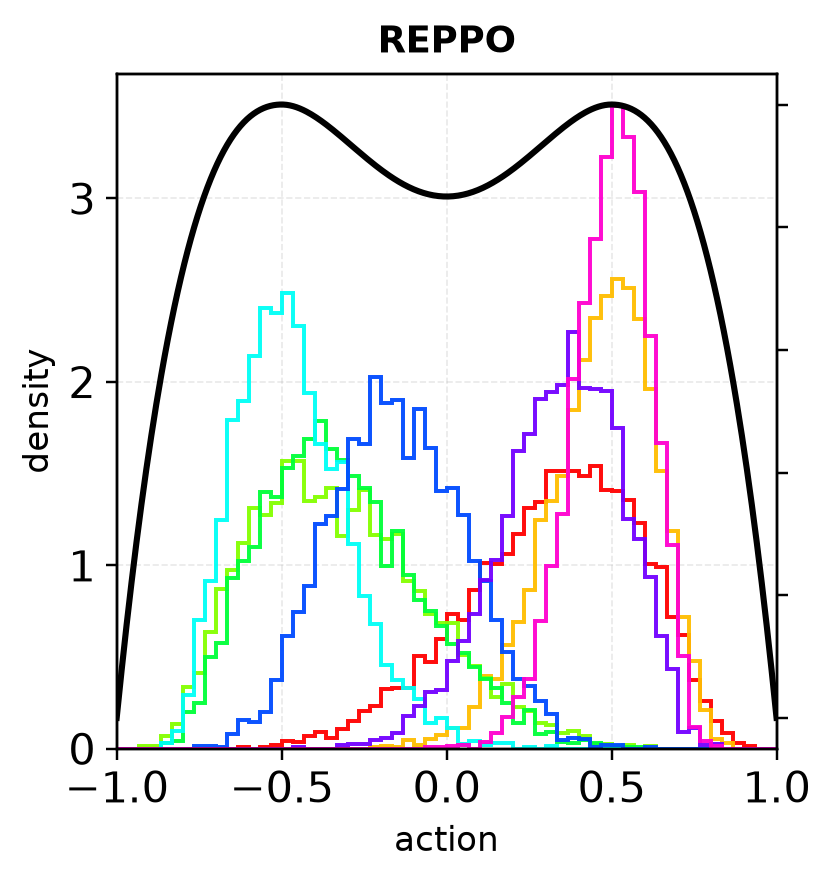
\includegraphics[height=0.59\textheight]
          {assets/multimodal_agent_reppo_histogram.png}%
      }
    \column{0.49\textwidth}
      \centering
      \uncover<2->{%
        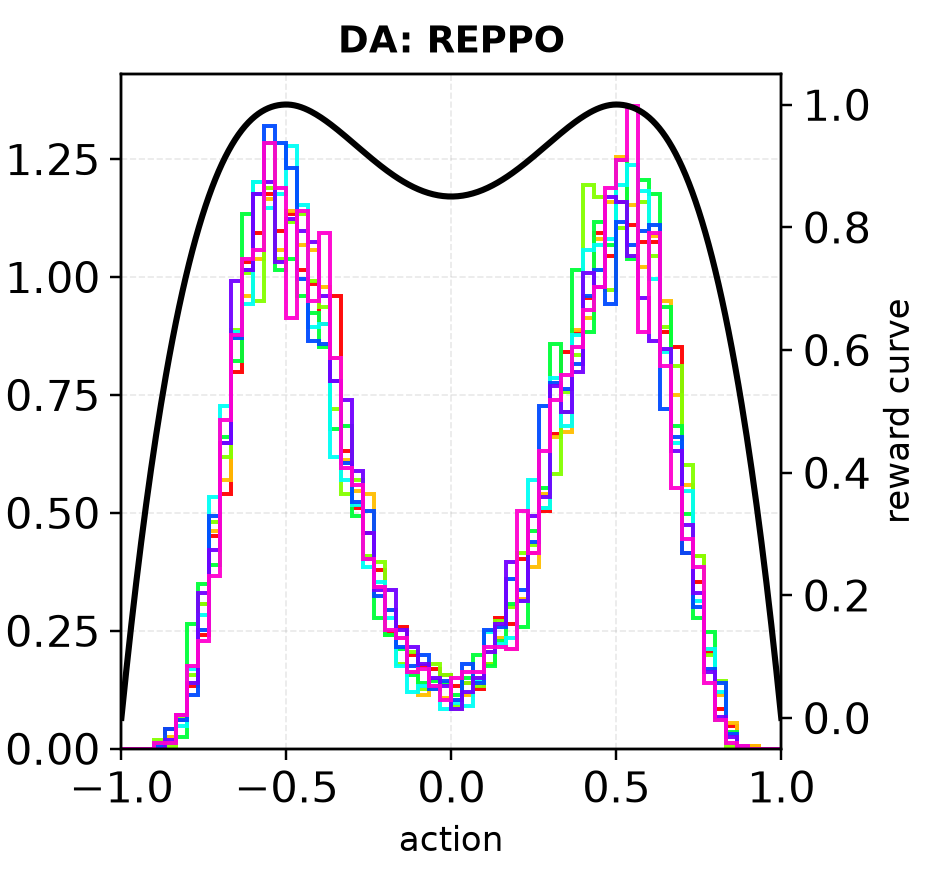
\includegraphics[height=0.59\textheight]
          {assets/multimodal_agent_da_reppo_histogram.png}%
      }
  \end{columns}
  \vspace{0.10cm}

  {\centering\multimodalstatelegend\par}
  \vspace{0.08cm}

  \uncover<3->{\small
    Each color denotes the same state in both panels. Gaussian REPPO selects
    one peak per state; DA-MDP: REPPO represents both optimal turns.}
\end{frame}

\begin{frame}{DA-MDP: recovered policy modes change behavior}
  \centering
  \begin{columns}[onlytextwidth]
    \column{0.49\textwidth}
      \centering\bfseries REPPO
    \column{0.49\textwidth}
      \centering\bfseries DA-MDP: REPPO
  \end{columns}
  \vspace{0.08cm}

  \animategraphics[autoplay,loop,poster=last,width=0.96\linewidth]
    {5}{assets/multimodal_agent_reppo_vs_da_reppo/frame-}{0}{25}
  \vspace{0.08cm}

  \small
  With the same benchmark and reward, REPPO drives all rollouts in one
  direction. DA-MDP: REPPO covers both action modes and produces diverse optimal
  trajectories.\quad
  \href{https://arxiv.org/abs/2512.02019}
    {\textcolor{BrandBlue}{Sanokowski \& Patil (2026)}}.
\end{frame}

\begin{frame}{References and course material}
  \scriptsize
  \begin{itemize}
    \item Sanokowski \& Patil (2026): \emph{Diffusion-Augmented MDPs}
    \item Kingma \& Welling (2014): \emph{Auto-Encoding Variational Bayes}
    \item Williams (1992): \emph{REINFORCE}
    \item Song et al. (2021): \emph{Score-Based Generative Modeling}
    \item Vargas, Grathwohl \& Doucet (2023): \emph{Denoising Diffusion Samplers}
    \item Levine (2018): \emph{RL and Control as Probabilistic Inference}
    \item \href{https://arxiv.org/abs/1801.01290}
      {\textcolor{BrandBlue}{Haarnoja et al. (2018): \emph{Soft Actor-Critic}}}
    \item \href{https://arxiv.org/abs/1502.05477}
      {\textcolor{BrandBlue}{Schulman et al. (2015): \emph{Trust Region Policy Optimization}}}
    \item \href{https://arxiv.org/pdf/2502.02316}
      {\textcolor{BrandBlue}{Celik et al. (2025):
      \emph{DIME: Diffusion-Based Maximum Entropy Reinforcement Learning}}}
    \item \href{https://arxiv.org/abs/2606.15260}
      {\textcolor{BrandBlue}{Le et al. (2026):
      \emph{Trust-Region Diffusion Policies for Massively Parallel On-Policy RL} (TruDi)}}
    \item Course folders:
      \texttt{L1-VariationalInference/}
      $\rightarrow$ \texttt{L2-DiffusionSamplers/}
  \end{itemize}
\end{frame}

\begin{frame}[plain]
  \begin{tikzpicture}[remember picture,overlay]
    \fill[BrandBlue] (current page.south west) rectangle (current page.north east);
    \path[fill=white,fill opacity=0.08]
      (current page.south west) -- (current page.north west)
      -- ([xshift=5.4cm]current page.north west)
      -- ([xshift=8.3cm]current page.south west) -- cycle;
    \node[anchor=west,align=left,text=white,text width=8.6cm]
      at ([xshift=1.05cm,yshift=0.10cm]current page.west)
      {{\bfseries\fontsize{34}{38}\selectfont Thank you!}\\[0.30cm]
       {\fontsize{17}{21}\selectfont Sebastian Sanokowski}\\[0.65cm]
       {\fontsize{15}{20}\selectfont Interested in working on DA-MDPs?\\[0.12cm]
        Feel free to contact me.}};
    \node[fill=white,rounded corners=6pt,inner sep=0.40cm,
          align=center,text=Ink]
      at ([xshift=-2.9cm,yshift=0.10cm]current page.east)
      {\href{https://www.linkedin.com/in/sebastian-sanokowski-0664451b7/}{%
         \qrcode[height=3.2cm]{https://www.linkedin.com/in/sebastian-sanokowski-0664451b7/}}\\[0.18cm]
       {\bfseries\large LinkedIn}\\[0.06cm]
       {\small Scan to connect}};
  \end{tikzpicture}
  \plainlogos
\end{frame}

\end{document}
